\documentclass[12pt, a4paper]{report}
\usepackage[utf8]{inputenc}
\usepackage[T5]{fontenc}
\usepackage[vietnamese]{babel}
\usepackage{minted}
\usepackage{graphicx}
\usepackage{caption} 
\usepackage{geometry}
\usepackage{hyperref} 
\usepackage{amsmath}
\usepackage{float}
\usepackage{booktabs}
\usepackage{longtable}
\usepackage{array}
\usepackage{multicol}
\usepackage{pdflscape}
\usepackage{setspace}
\usepackage{background}
\usepackage{natbib}
\usepackage{enumitem} 

\backgroundsetup{
    scale=1,
    color=black,
    opacity=1,
    angle=0,
    position=current page.center,
    contents={
\includegraphics[width=\paperwidth,height=\paperheight]{background.png}}
}

\hypersetup{
    colorlinks=true,
    linkcolor=black,
    citecolor=black,
    urlcolor=black
}

\geometry{a4paper, margin=1in}

\begin{document}

% ----- Trang bìa -----
\begin{titlepage}
\BgThispage
    \centering
    \textbf{\large HỌC VIỆN CÔNG NGHỆ BƯU CHÍNH VIỄN THÔNG}\\
    \textbf{\Large KHOA CÔNG NGHỆ THÔNG TIN I}\\
    \centerline{--------------------o0o--------------------}  
    \vspace{1cm}
    
\includegraphics[width=8cm]{logo.png}\\ % 
    \vspace{1cm}
{\Large \textbf{BÁO CÁO BÀI TẬP LỚN 1}}\\[0.5cm]
{\LARGE \textbf{NGÔN NGỮ LẬP TRÌNH PYTHON}}\\
\vfill
\begin{center}
\begin{tabular}{@{}l@{\hspace{2cm}}l}
\textbf{Giảng viên hướng dẫn:} & \textbf{Kim Ngọc Bách} \\
\textbf{Sinh viên:}            & \textbf{Vũ Thị Thu Duyên} \\
\textbf{Mã sinh viên:}         & \textbf{B23DCCE027} \\
\textbf{Lớp:}                  & \textbf{D23CQCEO6-B} \\
\textbf{Niên khóa:}            & \textbf{2023 - 2028} \\
\textbf{Hệ đào tạo:}           & \textbf{Đại học chính quy} \\
\end{tabular}
\end{center}
\vfill

    {\large Hà Nội, 2025}
\end{titlepage}
\backgroundsetup{contents={}}

\newgeometry{top=2.5cm,bottom=2cm,left=3cm,right=2cm} 

\begin{center}
	{\textbf{\Large{NHẬN XÉT CỦA GIẢNG VIÊN }}}
\end{center}

\dotfill \vspace{0.25cm} \par
\dotfill \vspace{0.25cm} \par
\dotfill \vspace{0.25cm} \par
\dotfill \vspace{0.25cm} \par
\dotfill \vspace{0.25cm} \par
\dotfill \vspace{0.25cm} \par
\dotfill \vspace{0.25cm} \par
\dotfill \vspace{0.25cm} \par
\dotfill \vspace{0.25cm} \par
\dotfill \vspace{0.25cm} \par
\dotfill \vspace{0.25cm} \par
\dotfill \vspace{0.25cm} \par
\dotfill \vspace{0.25cm} \par
\dotfill \vspace{0.25cm} \par
\dotfill \vspace{0.25cm} \par
\dotfill \vspace{0.25cm} \par
\dotfill \vspace{0.25cm} \par
\dotfill \vspace{0.25cm} \par
\dotfill
\vspace{1cm}

{\textbf{\large{Điểm: }}} \hspace{1.0cm}\textbf{( Bằng chữ:}  \hspace{2.5cm}\textbf{)}  



\begin{flushright}
	Hà Nội, ngày \hspace{0.75cm} tháng \hspace{0.75cm} năm 20...\hspace{0.75cm}
	
	{\textbf{\large{Giảng viên  }}} \hspace{2cm} \textcolor{white}{.}
\end{flushright}
\clearpage
\tableofcontents
\newpage
\listoffigures   
\newpage

\chapter{Thu thập dữ liệu thống kê cầu thủ ngoại hạng anh mùa 2024-2025 từ \href{http://fbref.com}{fbref.com}}
\author{} 
\date{}

% Chương 1 
\section{Giới thiệu}
Bài tập này yêu cầu xây dựng một chương trình Python để tự động thu thập dữ liệu thống kê chi tiết của các cầu thủ bóng đá tại giải Ngoại hạng Anh (English Premier League - EPL) mùa giải 2024-2025 từ trang web \texttt{fbref.com}.
Chương trình sẽ tạo ra hai tệp kết quả:
\begin{itemize}
\renewcommand{\labelitemi}{}
    \item \texttt{results.csv}: Chứa dữ liệu của các cầu thủ có tổng số phút thi đấu trong cả mùa giải (cho một hoặc nhiều CLB) lớn hơn 90 phút, theo yêu cầu cụ thể của bài tập này. 
    \item \texttt{results1.csv}: Chứa dữ liệu của các cầu thủ thi đấu hơn 90 phút cho một câu lạc bộ cụ thể trong mùa giải. Tệp này giữ lại các bản ghi riêng lẻ theo từng đội và sẽ là dữ liệu đầu vào quan trọng cho các bài tập phân tích và tổng hợp thống kê tiếp theo, nơi cần dữ liệu chi tiết theo từng lần khoác áo CLB của cầu thủ.
\end{itemize}
Dưới đây sẽ là phần mô tả quá trình thực hiện, bao gồm lựa chọn thư viện, quy trình cào dữ liệu và kết quả thu được.

\section{Lựa chọn thư viện}
Để thực hiện nhiệm vụ cào dữ liệu từ một trang web động và xử lý dữ liệu hiệu quả, các thư viện Python sau đã được lựa chọn:
\begin{itemize}
\renewcommand{\labelitemi}{}
    \item \textbf{Selenium}: Thư viện này được chọn làm công cụ chính để tương tác với trang web FBRef vì trang này sử dụng nhiều JavaScript để tải và hiển thị nội dung, đặc biệt là các bảng dữ liệu thống kê phức tạp. Không giống như thư viện \texttt{requests} (vốn chỉ lấy mã nguồn HTML tĩnh ban đầu do máy chủ gửi về và không thể thực thi JavaScript), \texttt{selenium} hoạt động bằng cách điều khiển một trình duyệt web thực sự (như Chrome hoặc Firefox) một cách tự động. Điều này cho phép script chờ đợi các yếu tố động (như bảng dữ liệu) được JavaScript tải xong và hiển thị đầy đủ, thực thi bất kỳ mã JavaScript nào trên trang, và truy cập vào cấu trúc HTML cuối cùng (DOM) đã được render hoàn chỉnh. Nếu chỉ dùng \texttt{requests}, có nguy cơ rất cao sẽ bỏ lỡ các bảng dữ liệu quan trọng hoặc chỉ nhận được dữ liệu không đầy đủ, vì chúng được tạo ra hoặc điền dữ liệu bởi JavaScript sau khi trang tải lần đầu. 
    \item \textbf{BeautifulSoup4 (bs4)}: Sau khi \texttt{selenium} tải xong trang và lấy được mã nguồn HTML, \texttt{BeautifulSoup} được sử dụng để phân tích cú pháp (parse) HTML đó. 
    Nó cung cấp các phương thức tiện lợi để điều hướng HTML, tìm kiếm các thẻ (tags), thuộc tính (attributes) cụ thể (như \texttt{id}, \texttt{class}, \texttt{data-stat}), và trích xuất nội dung văn bản một cách dễ dàng và hiệu quả. 
    \item \textbf{Pandas}: Đây là thư viện mạnh mẽ cho thao tác và phân tích dữ liệu
    \item \textbf{Json}: Tệp \texttt{config.json} chứa các cấu hình quan trọng như URL cơ sở, tên các chỉ số cần lấy, ID bảng dữ liệu tương ứng, thuộc tính \texttt{data-stat}, ngưỡng số phút tối thiểu, v.v. Thư viện \texttt{json} được dùng để đọc và phân tích cú pháp tệp cấu hình này, giúp mã nguồn chính trở nên gọn gàng, dễ đọc và dễ bảo trì hơn. Việc tách cấu hình ra giúp dễ dàng thay đổi các tham số hoặc cập nhật cấu trúc trang web mà không cần sửa đổi nhiều trong mã lệnh Python. 
    \item \textbf{Re (Regular Expressions)}: Được sử dụng để trích xuất ID duy nhất của cầu thủ từ các đường dẫn URL trong mã HTML (\texttt{/players/<player\_id>/}). ID này rất quan trọng để định danh và tổng hợp dữ liệu cho cùng một cầu thủ khi họ xuất hiện ở nhiều bảng thống kê khác nhau hoặc thi đấu cho nhiều CLB trong mùa giải. 
    \item \textbf{Time}: Được sử dụng để tạo độ trễ nhỏ (\texttt{time.sleep}) giữa các yêu cầu truy cập trang web, nhằm tránh việc gửi quá nhiều yêu cầu liên tục đến máy chủ FBRef, giảm nguy cơ bị chặn IP và thể hiện hành vi duyệt web "lịch sự".
    \item \textbf{Collections.defaultdict}: Cực kỳ hữu ích khi cần tổng hợp dữ liệu. Trong trường hợp một cầu thủ thi đấu cho nhiều câu lạc bộ trong cùng mùa giải (ví dụ: chuyển nhượng giữa mùa), họ sẽ xuất hiện nhiều lần trong bảng dữ liệu. \texttt{defaultdict} được dùng để tạo một cấu trúc dữ liệu cho phép cộng dồn số phút thi đấu (\texttt{Min}) của cầu thủ đó từ các dòng khác nhau, trước khi áp dụng bộ lọc số phút tối thiểu. 
\end{itemize}

\section{Quá trình cào dữ liệu (Web Scraping)}
Ý tưởng chính của script này là tự động hóa quá trình thu thập dữ liệu từ một nguồn web động (fbref.com) bằng cách kết hợp Selenium để mô phỏng hành vi của người dùng và BeautifulSoup để phân tích cấu trúc HTML. Dữ liệu cần lấy được xác định dựa trên cấu hình bên ngoài (\texttt{config.json}), cho phép linh hoạt lựa chọn các thống kê cần thiết từ nhiều bảng khác nhau trên trang.
Điểm mấu chốt trong việc xử lý dữ liệu là chương trình ban đầu định danh mỗi bản ghi thống kê riêng lẻ theo cặp (ID cầu thủ duy nhất hoặc tên, tên đội). Việc này là cần thiết để phân biệt chính xác dữ liệu của cùng một cầu thủ khi họ thi đấu cho các câu lạc bộ khác nhau trong cùng một mùa giải (ví dụ: sau khi chuyển nhượng), bởi trên fbref, cầu thủ có thể xuất hiện ở nhiều dòng khác nhau nếu họ đổi đội.
Sau đó, dữ liệu này được xử lý theo hai cách riêng biệt để tạo ra hai tệp CSV: 
\begin{itemize}
    \item \textbf{results1.csv}: Lọc trực tiếp từ dữ liệu chi tiết, giữ lại những bản ghi mà cầu thủ thi đấu > 90 phút cho CLB đó. 
    \item \textbf{results.csv}: Tổng hợp tổng số phút thi đấu của từng cầu thủ trên toàn mùa giải, sau đó lọc những cầu thủ có tổng số phút > 90 và xuất ra tất cả các bản ghi liên quan đến cầu thủ đó (kể cả những bản ghi dưới 90 phút cho một CLB cụ thể, miễn là tổng số phút đạt yêu cầu). 
\end{itemize}
\textbf{Quy trình cào dữ liệu được thực hiện theo các bước sau:}
\begin{enumerate}[label=\textbf{Bước \arabic*:}, leftmargin=*]
    \item \textbf{Tải cấu hình}: Chương trình bắt đầu bằng việc đọc tệp \texttt{config.json} để lấy các thông tin cần thiết như URL gốc của mùa giải EPL trên fbref, danh sách các chỉ số thống kê cần thu thập, ID của các bảng HTML chứa dữ liệu, thuộc tính \texttt{data-stat} tương ứng với từng chỉ số, ngưỡng số phút thi đấu tối thiểu (\texttt{min\_minutes}), tên tệp CSV đầu ra, và thứ tự các cột trong tệp kết quả.
    \item \textbf{Khởi tạo selenium}: Một trình duyệt web tự động (WebDriver) được khởi tạo bằng \texttt{selenium}.
    \item \textbf{Truy cập và tải trang}:
    \begin{itemize}[leftmargin=0em]
        \item Chương trình duyệt đến URL của bảng thống kê chính (\texttt{stats}) cho mùa giải EPL 2024-2025. 
        \item Sử dụng \texttt{WebDriverWait} để chờ cho đến khi bảng dữ liệu chính (\texttt{stats\_standard}) xuất hiện và có thể tương tác, đảm bảo rằng mọi dữ liệu tải bằng JavaScript đã được hiển thị. 
    \end{itemize}
    \item \textbf{Phân tích HTML ban đầu}: Mã nguồn HTML của trang đã tải hoàn chỉnh được lấy từ \texttt{selenium} và chuyển cho \texttt{BeautifulSoup} để phân tích cú pháp. 
    \item \textbf{Thu thập dữ liệu từ nhiều bảng}:
    \begin{itemize}[leftmargin=0em]
        \item Script được thiết kế để lấy dữ liệu từ nhiều loại bảng thống kê khác nhau trên fbref (Standard, Shooting, Passing, Defensive Actions, etc.), như được định nghĩa trong \texttt{STATS\_CONFIG} của tệp \texttt{config.json}. 
        \item Đối với mỗi loại thống kê, script xây dựng URL tương ứng (ví dụ: \texttt{.../stats/}, \texttt{.../shooting/}, \texttt{.../passing/}). 
        \item Script truy cập từng URL này bằng \texttt{selenium}, đợi bảng dữ liệu tương ứng tải xong, lấy HTML và dùng \texttt{BeautifulSoup} để phân tích.
        \item Lặp qua từng dòng (\texttt{<tr>}) trong phần thân (\texttt{<tbody>}) của bảng dữ liệu. 
    \end{itemize}
    \item \textbf{Trích xuất dữ liệu cầu thủ}: Với mỗi dòng (đại diện cho một cầu thủ trong bảng đó), script thực hiện: 
    \begin{itemize}[leftmargin=0em]
        \item Tìm ô chứa tên cầu thủ và trích xuất tên (\texttt{Player}) và ID duy nhất của cầu thủ (\texttt{player\_id}) từ liên kết hồ sơ cầu thủ bằng biểu thức chính quy (\texttt{re}). 
        \item Sử dụng hàm \texttt{safe\_get\_text}, \texttt{get\_nation\_code} và cấu hình \texttt{data-stat} từ \texttt{config.json} để trích xuất giá trị của từng chỉ số thống kê được yêu cầu cho cầu thủ đó.
        \item Hàm này đảm bảo trả về "N/a" nếu một ô dữ liệu không tồn tại hoặc trống. 
    \end{itemize}
    \item \textbf{Lưu trữ tạm thời}: Dữ liệu của mỗi cầu thủ từ mỗi bảng được lưu vào một dictionary, sau đó được thêm vào một danh sách tổng hợp (\texttt{scraped\_data}). 
    \item \textbf{Tổng hợp và Lọc Dữ liệu (2 luồng)}:
    \begin{itemize}[leftmargin=0em]
        \item Luồng 1: Tạo dữ liệu cho \texttt{results1.csv}
        \begin{itemize}
            \item Lặp qua \texttt{scraped\_data}. 
            \item Với mỗi bản ghi (ứng với một cầu thủ tại một đội), kiểm tra giá trị \texttt{Playing Time: minutes ('Min')}. 
            \item Nếu số phút > \texttt{MIN\_MINUTES}, định dạng lại các giá trị (dùng \texttt{format\_value}) và thêm dictionary của bản ghi này vào danh sách \sloppypar
            
            \texttt{single\_team\_over\_90\_list}.
        \end{itemize}
        \item Luồng 2: Tạo dữ liệu cho \texttt{results.csv}
        \begin{itemize}
            \item Sử dụng \texttt{collections.defaultdict} (\texttt{player\_minutes\_aggregate}) để nhóm các bản ghi theo \texttt{player\_id} (hoặc \texttt{player\_name} nếu ID không có). 
            \item Trong quá trình nhóm, cộng dồn số phút thi đấu (\texttt{Min}) để tính \texttt{total\_minutes} cho mỗi cầu thủ.
            \item Lọc \texttt{player\_minutes\_aggregate}, chỉ giữ lại những cầu thủ có \texttt{total\_minutes} > \texttt{MIN\_MINUTES}.
            \item Với mỗi cầu thủ đủ điều kiện, lặp qua \textit{tất cả} các bản ghi gốc (entries) của cầu thủ đó (từ các đội khác nhau nếu có). 
            \item Định dạng lại các giá trị cho từng bản ghi và thêm vào danh sách \sloppypar \texttt{final\_player\_list\_of\_dicts}. 
        \end{itemize}
    \end{itemize}
    \item \textbf{Định dạng và Sắp xếp}:
    \begin{itemize}[leftmargin=0em]
        \item Cả hai danh sách (\texttt{single\_team\_over\_90\_list} và \texttt{final\_player\_list\_of\_dicts}) được sắp xếp theo tên (first name) của cầu thủ theo thứ tự bảng chữ cái. 
        \item Đảm bảo tất cả các cột theo \texttt{COLUMN\_ORDER} đều tồn tại, điền "N/a" nếu thiếu (đã thực hiện trong bước định dạng ở Bước 6).
    \end{itemize}
    \item \textbf{Xuất ra CSV}:
    \begin{itemize}[leftmargin=0em]
        \item Chuyển danh sách \texttt{final\_player\_list\_of\_dicts} thành pandas DataFrame và lưu vào tệp \texttt{results.csv} (được đặt tên trong \texttt{config.json}). 
        \item Chuyển danh sách \texttt{single\_team\_over\_90\_list} thành pandas DataFrame và lưu vào tệp \texttt{results1.csv}. 
        \item Cả hai tệp CSV đều không bao gồm chỉ số dòng (index) của DataFrame và sử dụng encoding \texttt{utf-8-sig} để hiển thị ký tự đặc biệt đúng cách. 
    \end{itemize}
\end{enumerate}

\section{Kết quả}
Chương trình thực thi và tạo ra hai tệp CSV: 
\begin{itemize}
\renewcommand{\labelitemi}{}
    \item \texttt{results1.csv}: Đã thu thập dữ liệu thống kê cho 491 cầu thủ, mỗi người đạt trên 90 phút thi đấu cho một câu lạc bộ ở giải Ngoại hạng Anh (EPL) mùa 2024-2025. 
    \item \texttt{results.csv}: Đã thu thập dữ liệu thống kê cho 496 cầu thủ, mỗi người đạt trên 90 phút thi đấu trong cả mùa 2024-2025. 
\end{itemize}
Việc tạo ra \texttt{results1.csv} đảm bảo dữ liệu gốc (đã lọc sơ bộ theo tiêu chí phút/đội) có sẵn cho các bước xử lý tiếp theo, trong khi \texttt{results.csv} giải quyết yêu cầu trực tiếp của bài 1 này.  

\begin{figure}[h]
    \centering
    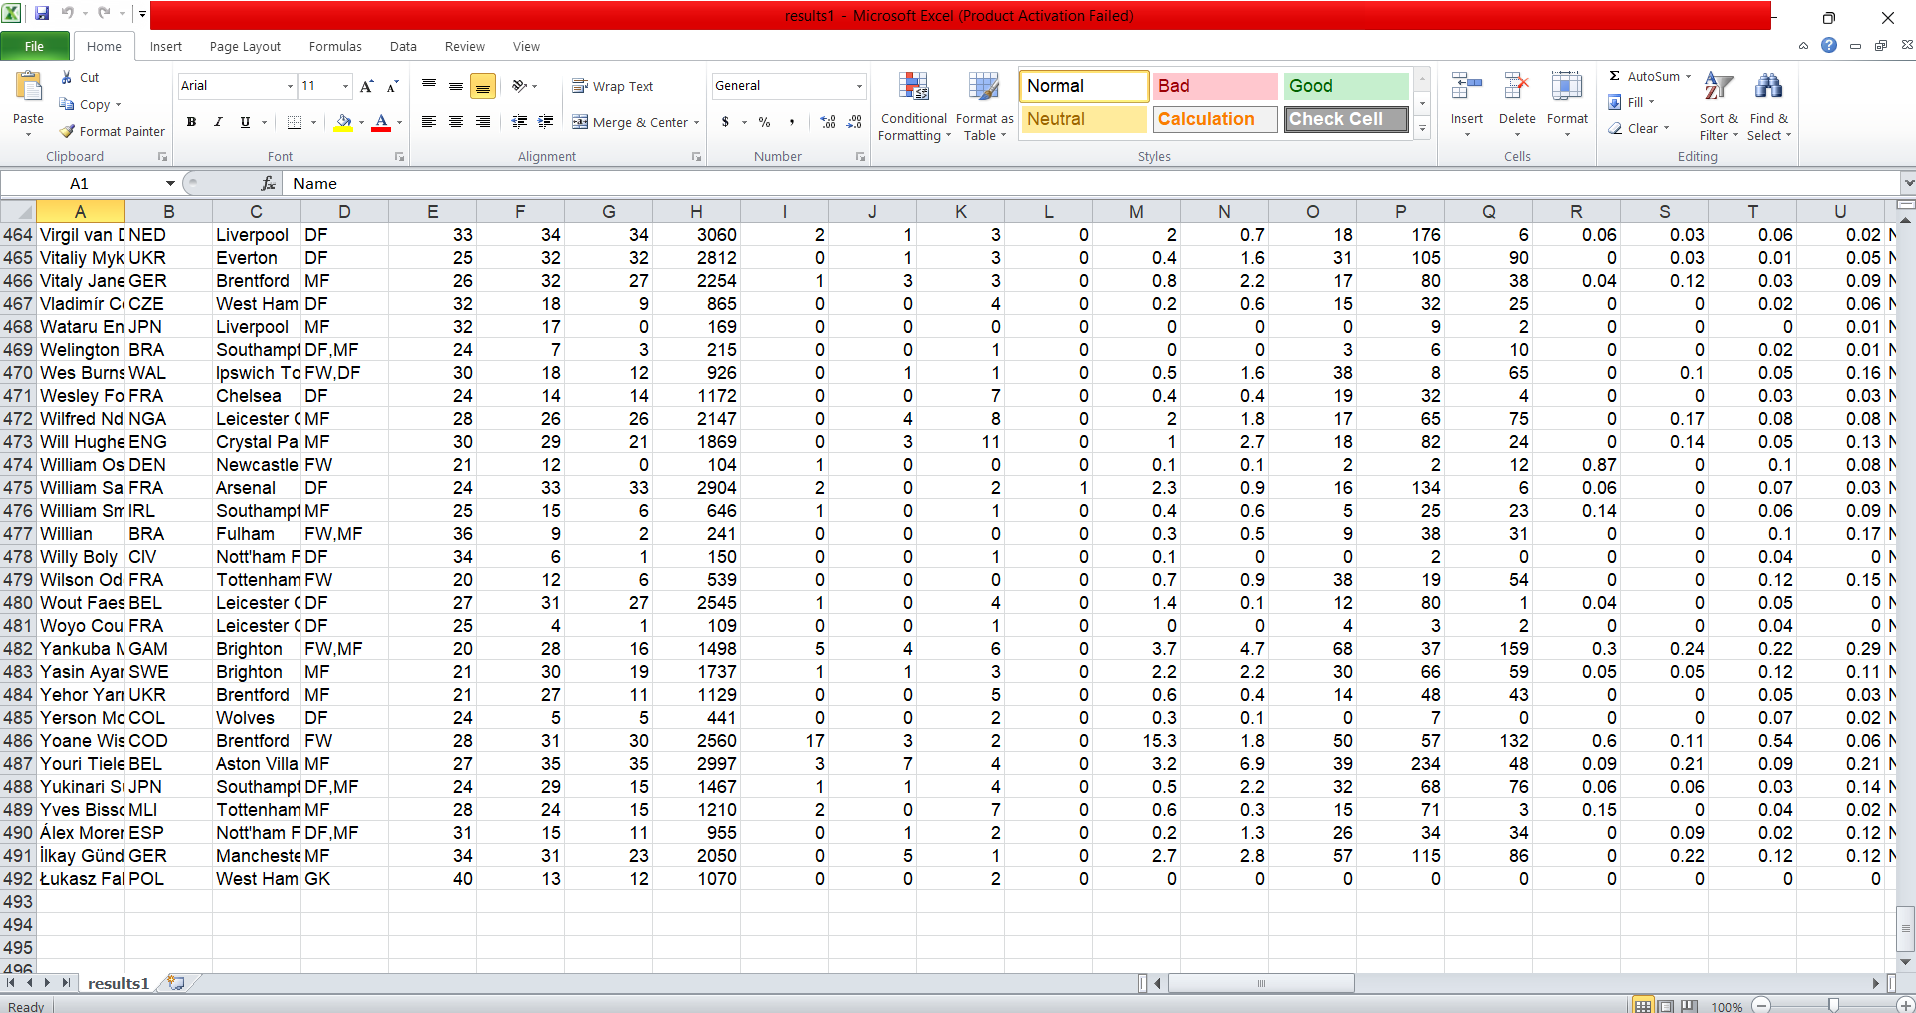
\includegraphics[width=\textwidth]{results.png}
    \caption{Hình ảnh file results.csv}
    \label{fig:results.csv}
\end{figure}
% Hết chương 1

% Chương 2
\chapter{Phân tích và trực quan hóa dữ liệu thống kê}

\section{Phân tích top 3 cầu thủ cao nhất và thấp nhất theo từng chỉ số thống kê}

\subsection{Khái quát về yêu cầu của bài toán}
Bài toán yêu cầu xử lý một tệp dữ liệu (\texttt{results1.csv} từ bài tập trước) chứa thông tin thống kê của các cầu thủ bóng đá.
Mục tiêu chính là xác định và liệt kê 3 cầu thủ có điểm số cao nhất (Top 3) và 3 cầu thủ có điểm số thấp nhất (Bottom 3) cho mỗi chỉ số thống kê có trong tệp dữ liệu.
Kết quả phân tích này được lưu vào một tệp văn bản có tên là \texttt{top\_3\_formatted.txt}.

\subsection{Khái quát logic code chính \newline (\texttt{top\_3\_statistical\_analysis.py})}
Script sử dụng thư viện \texttt{pandas} để đọc dữ liệu từ tệp CSV.
Sau đó, lặp qua từng cột thống kê (loại trừ các cột thông tin cơ bản như tên, quốc tịch, đội, vị trí).
Đối với mỗi cột thống kê, code cố gắng chuyển đổi dữ liệu sang dạng số, loại bỏ các giá trị không hợp lệ (\texttt{N/a} hoặc không thể chuyển đổi).
Nếu cột có thể được coi là số và có dữ liệu hợp lệ, code sẽ sắp xếp dữ liệu để tìm ra 3 giá trị cao nhất và 3 giá trị thấp nhất cùng với tên cầu thủ và đội tương ứng.
Cuối cùng, kết quả được định dạng và ghi vào tệp \texttt{top\_3\_formatted.txt}.

\subsection{Xử lý 'N/a'}
Trong quá trình xử lý dữ liệu, các giá trị \texttt{'N/a'} được xem là dữ liệu thiếu và được chuyển thành \texttt{NaN} thông qua tham số \texttt{na\_values=['N/a']} khi đọc file CSV bằng Pandas.
Ngoài ra, các giá trị không thể chuyển đổi sang dạng số cũng được ép về \texttt{NaN} bằng \texttt{pd.to\_numeric(errors='coerce')}.
Thay vì thay thế các giá trị thiếu bằng một con số cụ thể (như 0), toàn bộ các dòng chứa \texttt{NaN} ở cột cần đánh giá sẽ được loại bỏ trước khi thực hiện việc xếp hạng.
Việc này được thực hiện dựa trên các nguyên tắc sau:
\begin{itemize}
    \item \textbf{Tính đúng đắn của dữ liệu:} \texttt{NaN} thể hiện rằng dữ liệu bị thiếu hoặc không áp dụng, ví dụ như thông số dành riêng cho một vị trí cụ thể không phù hợp với cầu thủ ở vị trí khác. Việc thay thế bằng 0 sẽ làm sai lệch bản chất này.
    \item \textbf{Tránh gây hiểu nhầm:} Gán giá trị 0 cho dữ liệu thiếu có thể dẫn đến diễn giải sai – ví dụ, hiểu nhầm rằng cầu thủ không ghi bàn, trong khi thực tế dữ liệu chưa được ghi nhận.
    \item \textbf{Đảm bảo công bằng khi xếp hạng:} Việc chỉ xét các cầu thủ có dữ liệu hợp lệ giúp kết quả Top/Bottom 3 phản ánh đúng hiệu suất thực tế, tránh việc đưa các cá nhân thiếu dữ liệu vào so sánh một cách không chính xác.
\end{itemize}
Như vậy, việc giữ nguyên \texttt{NaN} và loại bỏ các giá trị thiếu khỏi quá trình xếp hạng là phương pháp hợp lý, đảm bảo tính khách quan và chính xác trong phân tích dữ liệu cầu thủ.

\subsection{Các bước thực thi}
\subsubsection*{Khởi tạo và chuẩn bị dữ liệu:}
Script nhập các thư viện cần thiết (\texttt{pandas}, \texttt{os}, \texttt{numpy}, \texttt{io}).
Đọc dữ liệu từ file \texttt{results.csv} vào DataFrame Pandas, cấu hình để xử lý \texttt{'N/a'} thành \texttt{NaN}.
Xác định danh sách các cột thống kê (\texttt{stats\_columns}) cần phân tích bằng cách loại trừ các cột định danh ('Name', 'Team', 'Position', 'Nation').

\subsubsection*{Xử lý từng cột và ghi file output:}
Mở file \texttt{top\_3\_formatted.txt} để ghi kết quả.
Script lặp qua từng cột \texttt{col} trong \texttt{stats\_columns}:
\begin{itemize}
    \item Ghi Tiêu đề Cột: Ghi tên cột hiện tại vào file.
    \item Chuẩn hóa \& Lọc Dữ liệu Số: Sử dụng \texttt{pd.to\_numeric(errors='coerce')} để ép kiểu cột \texttt{col} sang dạng số, chuyển lỗi thành \texttt{NaN}.
    \item Tạo DataFrame tạm \texttt{df\_for\_sort} và loại bỏ các hàng có giá trị \texttt{NaN} (\texttt{dropna()}) trong cột này.
    \item Bước này đảm bảo chỉ dữ liệu số, hợp lệ được sử dụng để xếp hạng.
    \item Xếp hạng và Ghi Kết quả:
    \begin{itemize}
        \item Nếu \texttt{df\_for\_sort} chứa dữ liệu số hợp lệ: Dùng \texttt{sort\_values()} để sắp xếp DataFrame này theo cột \texttt{col} giảm dần (tìm Top 3) và tăng dần (tìm Bottom 3), sau đó dùng \texttt{head(3)}.
        \item Kết quả (Tên, Đội, Chỉ số) và thông tin kiểu dữ liệu được ghi vào file.
    \end{itemize}
    \item Ghi Phân cách: Thêm dòng \texttt{===...} để phân tách kết quả giữa các cột.
\end{itemize}
Hoàn tất: Sau khi xử lý hết các cột, file \texttt{top\_3\_formatted.txt} được lưu lại, chứa toàn bộ kết quả phân tích.

\subsection{Kết quả (\texttt{top\_3\_formatted.txt})}
Tệp \texttt{top\_3\_formatted.txt} chứa kết quả phân tích cho từng chỉ số thống kê.
Mỗi chỉ số được trình bày rõ ràng với tiêu đề, tiếp theo là danh sách Top 3 và Bottom 3 cầu thủ.

\begin{figure}[H]
    \centering
    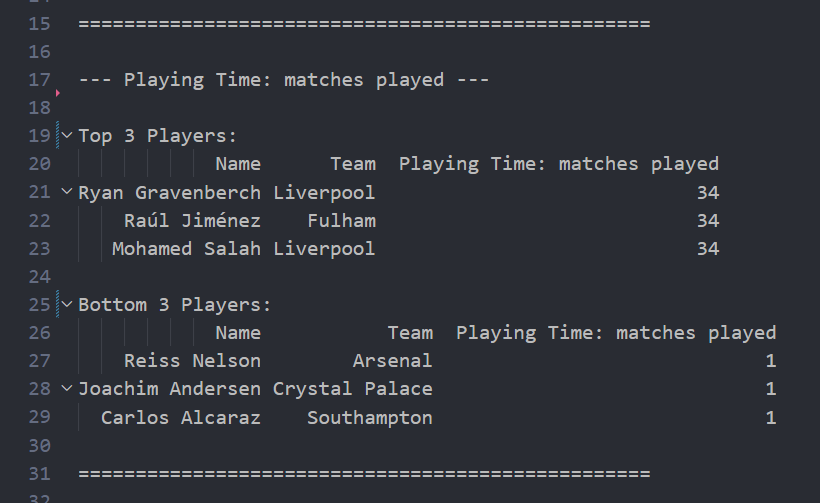
\includegraphics[width=0.8\textwidth]{top_3.png} 
    \caption{Ví dụ kết quả từ tệp top\_3\_formatted.txt.}
    \label{fig:top3_output}
\end{figure}

\section{Tính toán thống kê mô tả (median, mean, std dev) cho dữ liệu cầu thủ}

\subsection{Giới thiệu}
Bài tập này yêu cầu viết một chương trình Python để thực hiện các phép tính thống kê mô tả trên dữ liệu cầu thủ đã thu thập ở bài tập trước (\texttt{results1.csv}).
Cụ thể, chương trình cần tính toán:
\begin{itemize}
\renewcommand{\labelitemi}{}
    \item Giá trị trung vị (median) cho mỗi chỉ số thống kê trên toàn bộ tập dữ liệu.
    \item Giá trị trung bình (mean) và độ lệch chuẩn (standard deviation) cho mỗi chỉ số thống kê, tính toán trên toàn bộ tập dữ liệu và tính riêng cho từng đội (team).
\end{itemize}
Kết quả được lưu vào tệp \texttt{results2.csv} với một định dạng cụ thể, trong đó các hàng đại diện cho toàn bộ ('all') hoặc một đội cụ thể, và các cột đại diện cho các phép tính thống kê (Median, Mean, Std) áp dụng cho từng chỉ số.

\subsection{Lựa chọn thư viện}
\begin{itemize}[leftmargin=0em]
\renewcommand{\labelitemi}{}
    \item Thư viện \texttt{pandas}: Là thư viện chủ đạo, không thể thiếu cho tác vụ này.
    \item Thư viện \texttt{os}: Được sử dụng để quản lý đường dẫn tệp một cách linh hoạt và độc lập với hệ điều hành. \texttt{os.path.join} và \texttt{os.path.dirname} giúp xác định chính xác vị trí của tệp đầu vào (\texttt{results1.csv}) và tệp đầu ra (\texttt{results2.csv}) mà không cần mã hóa cứng đường dẫn.
\end{itemize}

\subsection{Logic và quy trình thực hiện}
Chương trình \texttt{calculating\_statistics.py} thực hiện các bước sau:
\begin{enumerate}[label=\textbf{Bước \arabic*:}, leftmargin=*]
    \item \textbf{Chuẩn bị và đọc dữ liệu:}
    Sử dụng \texttt{os} để xây dựng đường dẫn đến tệp input \texttt{results1.csv} và tệp output \texttt{results2.csv}.
    Đọc \texttt{results.csv} vào pandas DataFrame (\texttt{df}).
    Một danh sách \texttt{na\_values\_list} gồm nhiều biến thể của giá trị thiếu ('N/a', 'n/a', '', ...) được cung cấp cho tham số \texttt{na\_values} của \texttt{pd.read\_csv} để đảm bảo nhận diện đúng các giá trị này và chuyển đổi chúng thành \texttt{NaN} (Not a Number) của pandas, thuận lợi cho các phép tính sau này.
    \item \textbf{Xác định cột thống kê:}
    Định nghĩa danh sách \texttt{exclude\_cols} chứa các cột không phải là số liệu thống kê cần phân tích (ví dụ: 'Name', 'Nation', 'Team', 'Position', 'Age').
    Tạo danh sách \texttt{stats\_columns} bằng cách lọc các cột trong DataFrame, chỉ giữ lại những cột không nằm trong \texttt{exclude\_cols}.
    \item \textbf{Tính toán thống kê tổng thể ('all'):}
    Chọn các cột trong \texttt{stats\_columns} từ DataFrame \texttt{df}.
    Sử dụng phương thức \texttt{.agg(['median', 'mean', 'std'])} để tính đồng thời trung vị, trung bình và độ lệch chuẩn cho từng cột trong \texttt{stats\_columns}.
    Kết quả trả về có dạng các chỉ số thống kê là hàng, các cột gốc là cột.
    Sử dụng \texttt{.T} (transpose) để chuyển vị, đưa tên các chỉ số gốc (\texttt{stats\_columns}) thành chỉ số hàng, và 'median', 'mean', 'std' thành tên cột, lưu vào \texttt{overall\_stats}.
    Điều này giúp truy cập dễ dàng hơn ở bước sau.
    \item \textbf{Tính toán thống kê theo nhóm ('Team'):}
    Sử dụng \texttt{df.groupby('Team')} để nhóm DataFrame theo giá trị trong cột 'Team'.
    Trên đối tượng GroupBy này, chọn các cột \texttt{stats\_columns}.
    Áp dụng \texttt{.agg(['median', 'mean', 'std'])} để tính toán các chỉ số thống kê cho từng đội.
    Kết quả (\texttt{team\_stats}) sẽ có cấu trúc đa chỉ số (MultiIndex) ở cả hàng (Team) và cột (Statistic, Metric).
    \item \textbf{Tái cấu trúc dữ liệu cho đầu ra:}
    \begin{itemize}[leftmargin=0em]
        \item Tạo hàng 'all': Khởi tạo một DataFrame rỗng \texttt{all\_row} với chỉ số là 'all'. Lặp qua từng cột thống kê (\texttt{col} in \texttt{stats\_columns}), tạo ra các cột mới trong \texttt{all\_row} với tên theo định dạng \texttt{f'Median of \{col\}'}, \texttt{f'Mean of \{col\}'}, \texttt{f'Std of \{col\}'} và gán giá trị tương ứng lấy từ \texttt{overall\_stats} đã tính ở Bước 3.
        \item Tạo các hàng 'Team': Khởi tạo một DataFrame \texttt{team\_results} với chỉ số là tên các đội (lấy từ \texttt{team\_stats.index}). Lặp qua từng cột thống kê (\texttt{col} in \texttt{stats\_columns}), tạo ra các cột mới trong \texttt{team\_results} với tên định dạng tương tự như trên. Giá trị được lấy từ \texttt{team\_stats} bằng cách truy cập qua chỉ số đa cấp, ví dụ: \texttt{team\_stats[(col, 'median')]} để lấy cột trung vị của chỉ số \texttt{col}.
        \item Kết hợp Kết quả: Sử dụng \texttt{pd.concat([all\_row, team\_results])} để nối DataFrame chứa hàng 'all' và DataFrame chứa các hàng của từng đội lại với nhau theo chiều dọc, tạo thành DataFrame cuối cùng \texttt{final\_results} có cấu trúc đúng yêu cầu.
    \end{itemize}
    \item \textbf{Lưu Kết quả:}
    Xuất DataFrame \texttt{final\_results} ra tệp \texttt{results2.csv} bằng phương thức \texttt{.to\_csv()}.
    Tham số \texttt{index=True} được sử dụng (mặc định) để lưu chỉ số của DataFrame (chính là 'all' hoặc tên đội) vào cột đầu tiên của tệp CSV.
\end{enumerate}

\subsection{Kết quả}
Chương trình đã chạy thành công và tạo ra tệp \texttt{results2.csv}.
Tệp \texttt{results2.csv} chứa các kết quả thống kê tổng hợp theo định dạng yêu cầu:
\begin{itemize}
    \item Hàng: Hàng đầu tiên có chỉ số là 'all', đại diện cho thống kê trên toàn bộ cầu thủ. Các hàng tiếp theo có chỉ số là tên của từng đội, đại diện cho thống kê tính riêng cho cầu thủ của đội đó.
    \item Cột: Các cột được đặt tên theo mẫu "Metric of Statistic", ví dụ: "Median of Performance: goals", "Mean of Performance: goals", "Std of Performance: goals", "Median of Performance: assists", v.v., bao gồm tất cả các chỉ số trong \texttt{stats\_columns}.
    \item Giá trị: Các ô chứa giá trị trung vị, trung bình hoặc độ lệch chuẩn tương ứng đã được tính toán. Các giá trị NaN (nếu có, ví dụ: độ lệch chuẩn của nhóm chỉ có 1 cầu thủ) sẽ được biểu diễn dưới dạng ô trống trong tệp CSV.
\end{itemize}

\begin{figure}[H]
    \centering
    % Thay 'image_results2_csv_example.png' bằng tên file ảnh thực tế của bạn
    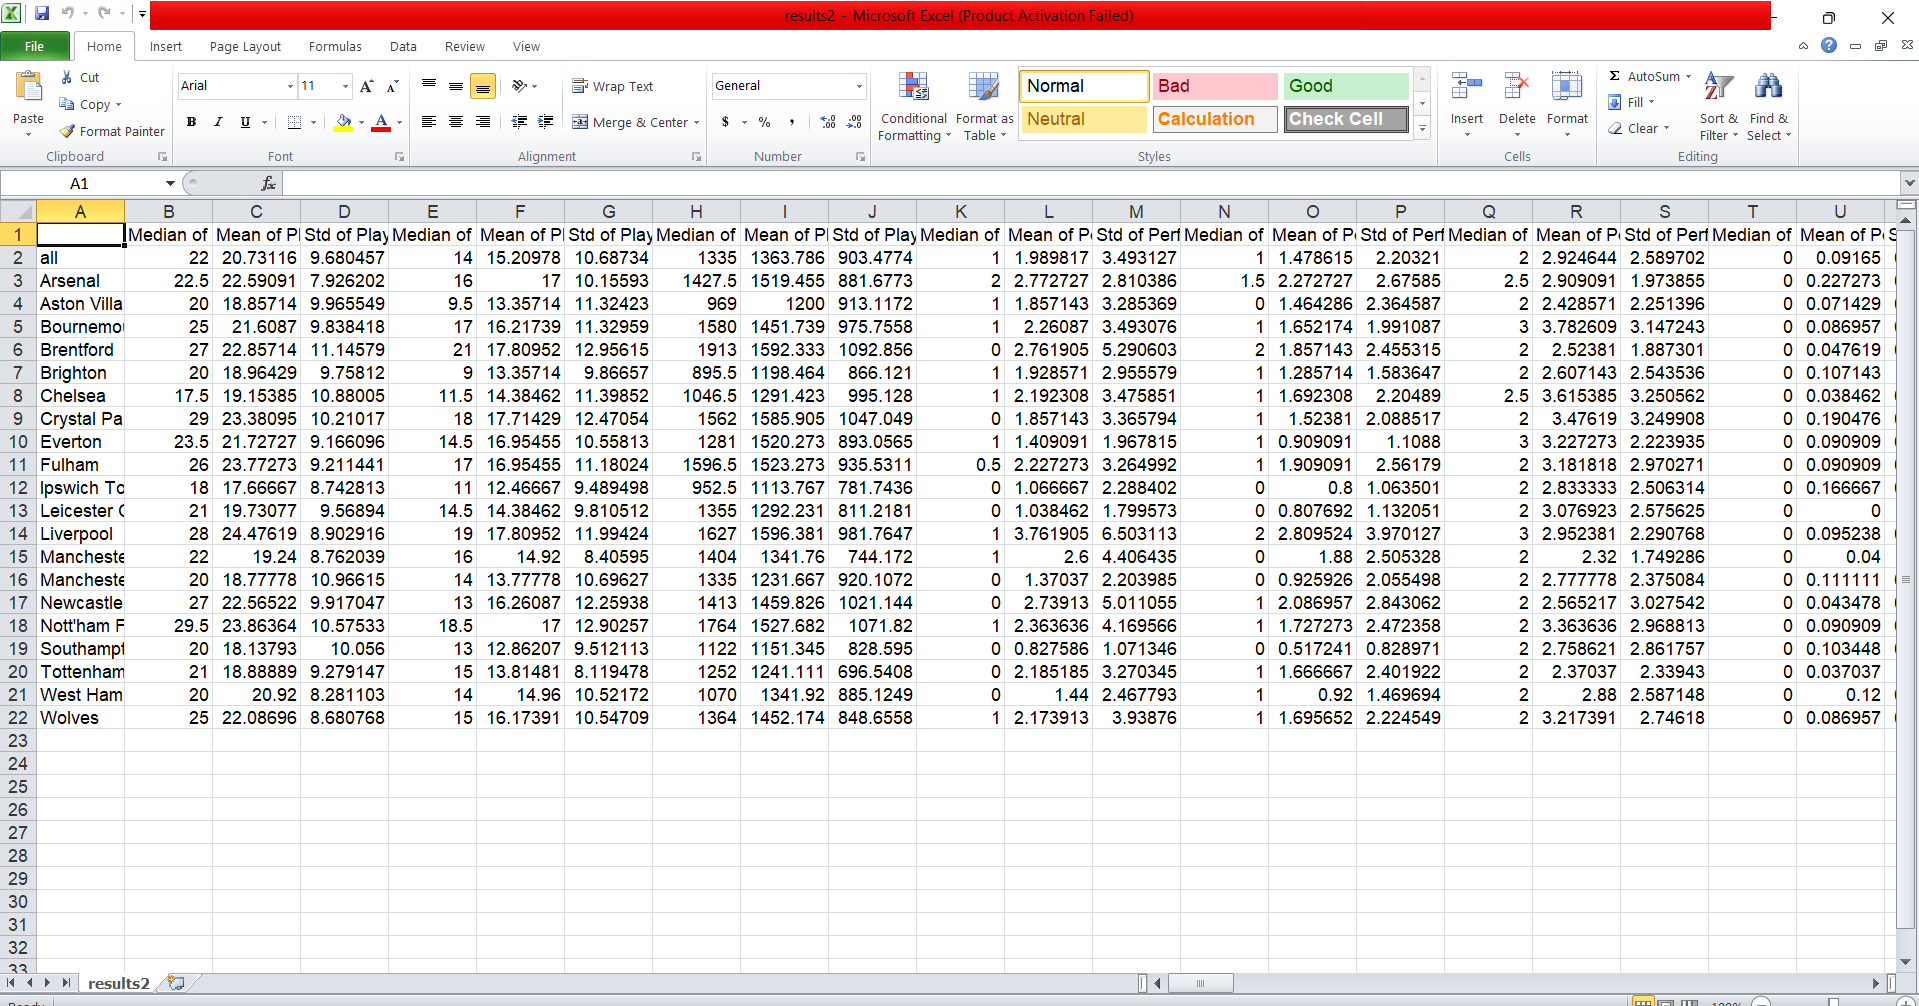
\includegraphics[width=\textwidth]{results2.png}
    \caption{Ví dụ dữ liệu từ tệp results2.csv.}
    \label{fig:results2_csv}
\end{figure}

\section{Trực quan hóa phân phối thống kê cầu thủ bằng biểu đồ histogram}

\subsection{Mục tiêu}
Mục tiêu chính của script \texttt{plot\_stat\_histograms.py} là trực quan hóa và phân tích sự phân phối của một tập hợp các chỉ số thống kê quan trọng của cầu thủ bóng đá.
Cụ thể, script nhằm:
\begin{itemize}
    \item Tạo biểu đồ histogram cho từng chỉ số thống kê được chọn (\texttt{stats\_to\_plot}) để thể hiện sự phân phối của chỉ số đó trên \textit{toàn bộ giải đấu} (tất cả cầu thủ).
    \item Tạo biểu đồ histogram riêng cho từng \textit{đội bóng}, thể hiện sự phân phối của từng chỉ số thống kê trong nội bộ đội đó.
    \item Lưu các biểu đồ này dưới dạng file ảnh (PNG) để dễ dàng xem xét, chia sẻ và phân tích sau này.
    \item Cung cấp cái nhìn trực quan về hình dạng phân phối (ví dụ: đối xứng, lệch trái, lệch phải), xu hướng trung tâm, và độ phân tán của các chỉ số thống kê, cả ở cấp độ giải đấu và cấp độ đội bóng.
\end{itemize}
Các chỉ số thống kê cụ thể được phân tích trong script này bao gồm: \texttt{'Performance: goals'}, \texttt{'Performance: assists'}, \texttt{'Standard: shoots on target percentage (SoT\%)'}, \texttt{'Blocks: Int'}, \texttt{'Performance: Recov'}, \texttt{'Challenges: Att'}.

\subsection{Lựa chọn Thư viện}
Script sử dụng một số thư viện Python phổ biến cho xử lý dữ liệu và trực quan hóa:
\begin{itemize}
    \item \texttt{pandas}: Thư viện cốt lõi để đọc dữ liệu từ file CSV (\texttt{results1.csv}), lưu trữ dữ liệu dưới dạng DataFrame, và thực hiện các thao tác xử lý, lọc, và lựa chọn dữ liệu cần thiết cho việc vẽ biểu đồ. Nó cũng xử lý các giá trị thiếu (NaN).
    \item \texttt{matplotlib.pyplot}: Thư viện nền tảng cho việc tạo biểu đồ trong Python. Nó được sử dụng để tạo khung hình (figure), các trục (axes), đặt tiêu đề, nhãn, và quản lý layout của biểu đồ, đặc biệt khi vẽ nhiều biểu đồ con (subplots) cho các đội.
    \item \texttt{seaborn}: Thư viện xây dựng trên \texttt{matplotlib}, cung cấp giao diện cấp cao hơn để vẽ các biểu đồ thống kê hấp dẫn và giàu thông tin. Cụ thể, \texttt{seaborn.histplot} được dùng để vẽ biểu đồ histogram, bao gồm cả đường ước lượng mật độ xác suất giúp làm mịn và hình dung rõ hơn hình dạng phân phối (KDE - Kernel Density Estimate). \texttt{seaborn.set\_theme} dùng để thiết lập phong cách thẩm mỹ chung cho các biểu đồ.
    \item \texttt{numpy}: Thư viện tính toán khoa học, được sử dụng trong hàm \texttt{calculate\_fd\_bins} để thực hiện các phép toán cần thiết (như căn bậc ba \texttt{np.cbrt}, logarit cơ số 2 \texttt{np.log2}) cho việc tính toán số lượng bins tối ưu theo quy tắc Freedman-Diaconis và Sturges.
    \item \texttt{os}: Thư viện cung cấp các hàm tương tác với hệ điều hành, chủ yếu được dùng để quản lý đường dẫn file (lấy đường dẫn thư mục hiện tại, nối đường dẫn), tạo thư mục lưu trữ (\texttt{stat\_histograms}), và đảm bảo đường dẫn hợp lệ.
    \item \texttt{math}: Thư viện toán học cơ bản, được sử dụng cho các hàm như \texttt{math.ceil} để làm tròn lên khi tính toán số lượng hàng/cột cho subplot và số lượng bins.
\end{itemize}

\subsection{Các bước thực hiện}
Script thực hiện các bước chính sau:
\subsubsection*{Thiết lập cấu hình}
Định nghĩa các hằng số như thư mục đầu ra (\texttt{OUTPUT\_DIR}), tên cột chứa thông tin đội (\texttt{TEAM\_COL}), số lượng đội tối đa trên mỗi biểu đồ (\texttt{TEAMS\_PER\_PLOT}), phong cách biểu đồ (\texttt{PLOT\_STYLE}), và giới hạn số bins tối đa (\texttt{MAX\_FD\_BINS}).

\subsubsection*{Định nghĩa hàm hỗ trợ}
\begin{itemize}
    \item \texttt{ensure\_dir}: Đảm bảo thư mục đầu ra tồn tại.
    \item \texttt{sanitize\_filename}: Làm sạch tên chỉ số thống kê để tạo tên file hợp lệ.
    \item \texttt{calculate\_fd\_bins}: Tính số lượng bins tối ưu cho histogram dựa trên quy tắc Freedman-Diaconis (ưu tiên) hoặc Sturges (dự phòng), giúp biểu đồ phản ánh tốt hơn cấu trúc dữ liệu thực tế và tránh việc chọn số bins tùy tiện. Có giới hạn số bins tối đa để tránh quá chi tiết.
\end{itemize}

\subsubsection*{Định nghĩa hàm vẽ biểu đồ}
\begin{itemize}
    \item \texttt{plot\_overall\_hist}:
    \begin{itemize}
        \item Nhận DataFrame, tên chỉ số thống kê, và thư mục đầu ra.
        \item Lọc dữ liệu cho chỉ số thống kê, chuyển đổi sang dạng số và loại bỏ giá trị thiếu (\texttt{NaN}).
        \item Tính số bins tối ưu bằng \texttt{calculate\_fd\_bins}.
        \item Sử dụng \texttt{seaborn.histplot} để vẽ histogram phân phối tổng thể, bật KDE.
        \item Đặt tiêu đề, nhãn trục và lưu biểu đồ vào file PNG với tên được chuẩn hóa.
    \end{itemize}
    \item \texttt{plot\_team\_hist}:
    \begin{itemize}
        \item Nhận DataFrame, tên chỉ số, thư mục đầu ra, tên cột đội, và số đội trên mỗi hình.
        \item Lấy danh sách các đội duy nhất và chia thành các nhóm nhỏ \sloppypar
    (theo \texttt{TEAMS\_PER\_PLOT}).
        \item Lặp qua từng nhóm đội:
        \begin{itemize}
            \item Tạo một figure mới với các subplots (lưới biểu đồ con).
            \item Lọc dữ liệu chỉ chứa các đội trong nhóm hiện tại.
            \item Tính số bins tối ưu \textit{dựa trên phạm vi dữ liệu của các đội trong nhóm này}. Điều này giúp các histogram trong cùng một figure có cùng cách chia khoảng giá trị.
            \item Xác định giới hạn trục x (\texttt{x\_min}, \texttt{x\_max}) chung cho tất cả các subplot trong figure hiện tại để dễ so sánh.
            \item Vẽ histogram cho từng đội trên một subplot riêng biệt bằng \texttt{seaborn.histplot}, sử dụng số bins và phạm vi bin (\texttt{binrange}) đã tính.
            \item Đặt tiêu đề con là tên đội, ẩn nhãn trục để tránh rối mắt, giới hạn trục x thống nhất.
            \item Ẩn các subplot thừa.
            \item Đặt tiêu đề chính cho figure (bao gồm tên chỉ số và nhóm đội).
            \item Lưu figure chứa histogram của nhóm đội vào file PNG.
        \end{itemize}
    \end{itemize}
\end{itemize}

\subsubsection*{Hàm thực thi chính (\texttt{if \_\_name\_\_ == '\_\_main\_\_':})}
\begin{itemize}
    \item Thiết lập theme cho \texttt{seaborn}.
    \item Định nghĩa danh sách các chỉ số cần vẽ (\texttt{stats\_to\_plot}).
    \item Xác định đường dẫn và đọc file \texttt{results.csv} vào DataFrame.
    \item Đảm bảo thư mục đầu ra tồn tại.
    \item Lặp qua từng chỉ số trong \texttt{stats\_to\_plot}:
    \begin{itemize}
        \item Gọi \texttt{plot\_overall\_hist} để vẽ biểu đồ tổng thể.
        \item Gọi \texttt{plot\_team\_hist} để vẽ biểu đồ cho từng đội (được nhóm lại).
    \end{itemize}
\end{itemize}

\subsection{Kết quả trực quan}
Kết quả đầu ra của script là một tập hợp các file ảnh PNG được lưu trong thư mục \texttt{stat\_histograms}.
Cụ thể:
\begin{itemize}
    \item Với mỗi chỉ số thống kê trong \texttt{stats\_to\_plot}, sẽ có \textit{một file} biểu đồ histogram thể hiện phân phối tổng thể của chỉ số đó trên toàn giải đấu \sloppypar
    (ví dụ: \texttt{hist\_overall\_Standard\_shoots\_on\_target\_percentage\_SoT.png}).
\end{itemize}

\begin{figure}[H]
    \centering
    % Thay 'image_hist_overall_sot.png' bằng tên file ảnh thực tế của bạn
    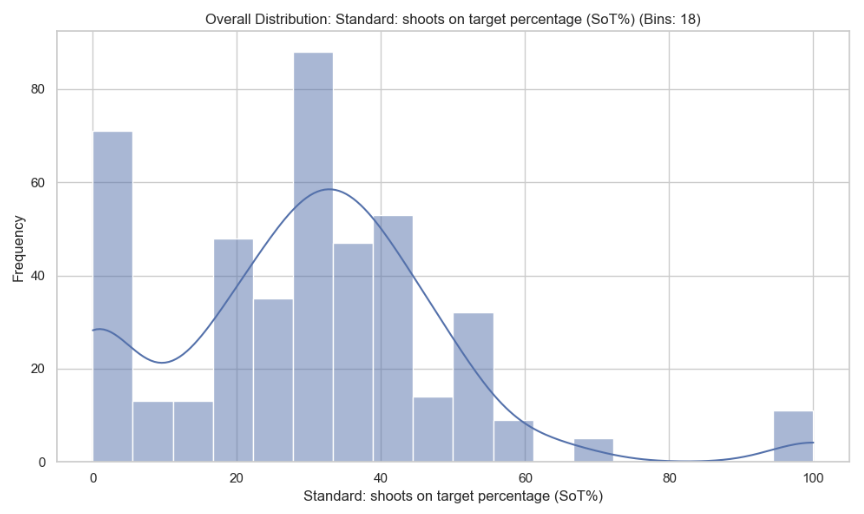
\includegraphics[width=0.8\textwidth]{overall.png}
    \caption{Ví dụ biểu đồ histogram tổng thể (Nguồn: Trích từ tài liệu gốc).}
    \label{fig:hist_overall_sot}
\end{figure}

\begin{itemize}
    \item Với mỗi chỉ số thống kê, sẽ có \textit{một hoặc nhiều file} biểu đồ histogram thể hiện phân phối của chỉ số đó theo từng đội. Các đội được nhóm lại (mặc định 20 đội/hình) để tránh tạo quá nhiều file hoặc hình ảnh quá lớn \sloppypar
    (ví dụ: \texttt{hist\_teams\_tandard\_shoots\_on\_target\_percentage\_SoT\_group\_1.png},...).
\end{itemize}

\begin{figure}[H]
    \centering
    % Thay 'image_hist_teams_sot_group1.png' bằng tên file ảnh thực tế của bạn
    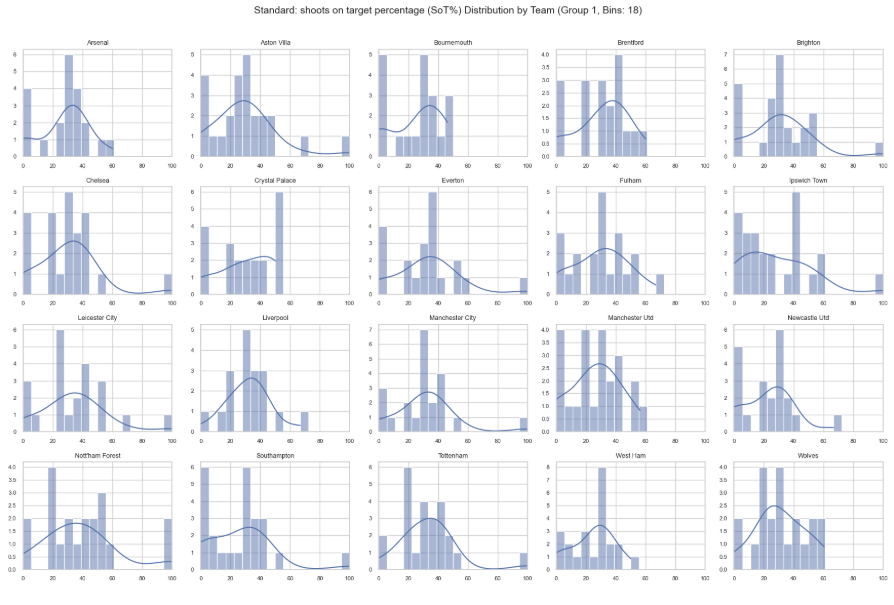
\includegraphics[width=\textwidth]{by_team.png}
    \caption{Ví dụ biểu đồ histogram theo nhóm đội (Nguồn: Trích từ tài liệu gốc).}
    \label{fig:hist_teams_sot_group1}
\end{figure}

Mỗi file này chứa một lưới các biểu đồ nhỏ, mỗi biểu đồ nhỏ tương ứng với một đội.
Các biểu đồ này cho phép người xem quan sát trực quan hình dạng phân phối (đối xứng, lệch, đa đỉnh), phạm vi giá trị, và tần suất xuất hiện của các giá trị khác nhau cho từng chỉ số, cả trên tổng thể và trong từng đội.

\subsection{Hạn chế}
Trong quá trình phân tích dữ liệu thống kê cầu thủ, biểu đồ histogram được sử dụng để trực quan hóa phân phối của từng chỉ số (ví dụ: số bàn thắng, số phút thi đấu, số pha kiến tạo, v.v.).
Đây là công cụ hiệu quả giúp quan sát nhanh xu hướng phổ biến, phát hiện các giá trị ngoại lai (outliers) và so sánh sự khác biệt giữa các cầu thủ hoặc đội bóng.
Tuy nhiên, việc sử dụng histogram cũng tồn tại một số điểm hạn chế cần được lưu ý để tránh đưa ra các kết luận thiếu chính xác hoặc phiến diện:
\begin{itemize}
    \item \textbf{Phụ thuộc vào chất lượng dữ liệu:} Kết quả trực quan hoàn toàn phụ thuộc vào tính đầy đủ và chính xác của dữ liệu trong file \texttt{results.csv}. Các giá trị thiếu (\texttt{NaN}) đã bị loại bỏ trong quá trình xử lý để đảm bảo tính chính xác của biểu đồ. Tuy nhiên, nếu tỷ lệ dữ liệu thiếu lớn hoặc không phân bố ngẫu nhiên, điều này có thể làm sai lệch hình dạng phân phối và dẫn đến nhận định thiếu khách quan về xu hướng tổng thể.
    \item \textbf{Nhạy cảm với số lượng Bins:} Mặc dù số lượng bins được xác định dựa trên quy tắc Freedman-Diaconis nhằm tối ưu hóa mức độ chi tiết của biểu đồ, histogram vẫn có thể thay đổi hình dạng nếu thay đổi số lượng bins. Bên cạnh đó, việc đặt giới hạn tối đa cho số bins (qua biến \texttt{MAX\_FD\_BINS}) mang tính chủ quan và có thể ảnh hưởng đến mức độ phân giải của biểu đồ, đặc biệt trong các phân phối có nhiều giá trị phân tán.
\end{itemize}

\section{Phân tích hiệu suất các đội bóng Premier League 2024–2025}

\subsection{Giới thiệu}
Nhằm đánh giá hiệu suất thi đấu của các đội bóng tại mùa giải 2024–2025, quá trình phân tích được thiết kế với hai mục tiêu chính: xác định đội dẫn đầu ở từng chỉ số thống kê và tìm ra đội có hiệu suất tổng thể tốt nhất.
Việc xử lý dữ liệu được thực hiện thông qua hai tệp chính:
\begin{itemize}
    \item \texttt{highest\_stats\_team.py}: Tệp mã nguồn Python đảm nhận toàn bộ quy trình phân tích, từ việc đọc dữ liệu, phân loại các chỉ số (tốt, xấu, bỏ qua), xác định đội dẫn đầu theo từng tiêu chí, đến tổng hợp kết quả để xác định đội xuất sắc nhất mùa giải.
    \item \texttt{config.json}: Tệp cấu hình cho phép tùy chỉnh linh hoạt các tham số như đường dẫn dữ liệu, cách xử lý giá trị thiếu và hệ thống phân loại chỉ số. Việc tách riêng cấu hình giúp điều chỉnh tiêu chí phân tích mà không cần sửa đổi mã nguồn.
\end{itemize}
Cách tiếp cận này giúp tối ưu hóa khả năng tái sử dụng, dễ bảo trì và mở rộng cho các mùa giải hoặc bộ dữ liệu khác nhau.

\subsection{Ý tưởng chính}
\begin{itemize}[leftmargin=0em]
\renewcommand{\labelitemi}{}
    \item \textbf{Xác định đội có điểm cao nhất cho mỗi chỉ số:} script phân loại các chỉ số thành ba nhóm (tốt, xấu, bỏ qua) dựa trên file cấu hình (\texttt{config.json}). Với mỗi chỉ số, code chuyển đổi dữ liệu thành dạng số, sau đó tìm giá trị tối ưu (cao nhất cho chỉ số tốt, thấp nhất cho chỉ số xấu) và xác định đội nào đạt được giá trị đó. Ví dụ, đội có nhiều bàn thắng nhất, đội có tỷ lệ chuyền bóng thành công cao nhất, hoặc đội có ít thẻ đỏ nhất.
    \item \textbf{Xác định đội có hiệu suất tổng thể tốt nhất:} Code đếm số lần mỗi đội dẫn đầu ở các chỉ số khác nhau, tính riêng cho chỉ số tốt và chỉ số xấu. Sau đó, tính tổng điểm kết hợp cho mỗi đội bằng cách cộng số lần dẫn đầu ở cả hai loại chỉ số. Đội có tổng số lần dẫn đầu nhiều nhất được coi là đội có hiệu suất tổng thể tốt nhất trong mùa giải.
\end{itemize}

\subsection{Quy trình thực thi}
Quy trình phân tích được điều khiển bởi tập lệnh \texttt{highest\_stats\_team.py}, với các bước chính sau:
\subsubsection*{Khởi tạo \& tải cấu hình}
Tải cấu hình từ \texttt{config.json} bằng hàm \texttt{load\_config}. Hàm này đọc tệp JSON và tạo các tập hợp (set) từ khóa \texttt{ignore\_stats\_set}, \texttt{bad\_stats\_set}, \texttt{good\_stats\_set} để phân loại chỉ số.

\subsubsection*{Xác định đường dẫn \& đọc dữ liệu CSV}
Xây dựng đường dẫn tuyệt đối đến tệp \texttt{results2.csv} (nằm trong \sloppypar
\texttt{../calculating\_statistics/}).
Đọc dữ liệu từ CSV vào DataFrame \texttt{dataframe} bằng \texttt{pandas}, sử dụng \texttt{na\_values} từ config.

\subsubsection*{Tiền xử lý DataFrame}
Xác định cột tên đội (mặc định là cột đầu tiên).
Chuẩn hóa cột tên đội: chuyển sang chữ thường, loại bỏ các hàng có tên đội là "all".

\subsubsection*{Xác định đội dẫn đầu cho mỗi chỉ số thống kê hợp lệ \sloppypar
(Hàm \texttt{analyze\_performance\_by\_stat\_type})}
\begin{enumerate}[label*=\textbf{Bước \arabic*:}, leftmargin=*]
    \item Xác định và Lọc Chỉ số cần Phân tích:
    \begin{itemize}[leftmargin=0em]
        \item Tạo danh sách các cột có tiền tố "Mean of " (trừ cột đội).
        \item Với mỗi cột tiềm năng:
        \begin{itemize}
            \item Trích xuất tên chỉ số thực (bỏ "Mean of ").
            \item Phân loại chỉ số (dùng \texttt{classify\_stat}) thành 'ignore', 'bad', 'good', hoặc 'uncategorized' dựa trên các tập hợp từ khóa đã tải.
            \item Nếu không phải 'ignore', chuyển cột sang dạng số. Chỉ giữ lại các chỉ số có ít nhất một giá trị số hợp lệ.
        \end{itemize}
    \end{itemize}
    \item Phân tích từng Chỉ số đã Lọc:
    \begin{itemize}[leftmargin=0em]
        \item Với mỗi chỉ số được chọn để phân tích:
        \begin{itemize}
            \item Chuyển cột chỉ số sang dạng số và loại bỏ các giá trị không hợp lệ (\texttt{NaN}).
            \item Tìm giá trị tốt nhất:
            \begin{itemize}
                \item Nếu loại là 'good' hoặc 'uncategorized': tìm giá trị \textit{lớn nhất}.
                \item Nếu loại là 'bad': tìm giá trị \textit{nhỏ nhất}.
            \end{itemize}
            \item Nếu không tìm thấy giá trị tốt nhất (ví dụ: cột rỗng), ghi nhận lỗi.
            \item Ngược lại:
            \begin{itemize}
                \item Xác định (các) đội đạt được giá trị tốt nhất này.
                \item Lưu tên (các) đội dẫn đầu, giá trị tốt nhất (ở dạng gốc để hiển thị) và loại chỉ số vào một dictionary kết quả.
            \end{itemize}
        \end{itemize}
    \end{itemize}
    \item Trả về: Dictionary chứa kết quả phân tích cho từng chỉ số.
\end{enumerate}

\subsubsection*{Hiển thị kết quả phân tích chi tiết}
Sắp xếp kết quả theo tên chỉ số.
Lặp qua từng chỉ số đã phân tích, định dạng giá trị (dùng \texttt{format\_value} để xử lý số nguyên, số thực, "N/A") và in ra: tên chỉ số, loại (GOOD, BAD), đội dẫn đầu, giá trị đạt được.

\subsubsection*{Tính toán và hiển thị bảng xếp hạng tổng Hợp}
\begin{enumerate}[label*=\textbf{Bước \arabic*:}, leftmargin=*]
    \item Đếm số lần dẫn đầu:
    \begin{itemize}[leftmargin=0em]
        \item Với mỗi chỉ số có kết quả hợp lệ trong \texttt{analysis\_results}:
        \begin{itemize}
            \item Nếu đội dẫn đầu chỉ số 'good', tăng điểm cho đội đó trong \texttt{good\_lead\_counts}.
            \item Nếu đội dẫn đầu chỉ số 'bad', tăng điểm cho đội đó trong \texttt{bad\_lead\_counts}.
        \end{itemize}
    \end{itemize}
    \item Tạo điểm tổng hợp:
    \begin{itemize}[leftmargin=0em]
        \item Lấy danh sách tất cả các đội duy nhất từ DataFrame.
        \item Khởi tạo điểm 0 cho tất cả các đội.
        \item Cộng tổng số lần dẫn đầu 'good' và 'bad' để có điểm tổng hợp cho mỗi đội.
    \end{itemize}
    \item Sắp xếp và Hiển thị:
    \begin{itemize}[leftmargin=0em]
        \item Sắp xếp các đội: giảm dần theo điểm tổng hợp, sau đó tăng dần theo tên đội (nếu cùng điểm).
        \item In bảng xếp hạng với thứ hạng, tên đội và tổng số lần dẫn đầu.
    \end{itemize}
\end{enumerate}

\subsection{Kết quả}
Khi script \texttt{highest\_stats\_team.py} được thực thi thành công, nó sẽ tạo ra hai khối thông tin chính được in ra console (màn hình dòng lệnh).
Các kết quả này cung cấp một cái nhìn chi tiết về hiệu suất của từng đội đối với mỗi chỉ số thống kê được phân tích, và một bảng xếp hạng tổng hợp các đội dựa trên số lần họ dẫn đầu các chỉ số đó.

\begin{figure}[H]
    \centering
    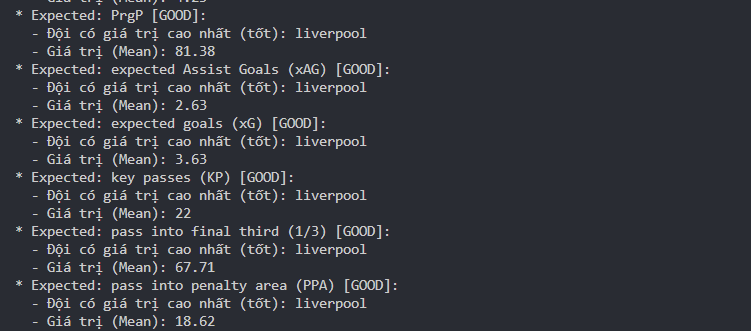
\includegraphics[width=0.8\textwidth]{output_2.4.1.png}
    \caption{Ví dụ kết quả phân tích chi tiết theo chỉ số.}
    \label{fig:analysis_output1}
\end{figure}

\begin{figure}[H]
    \centering
    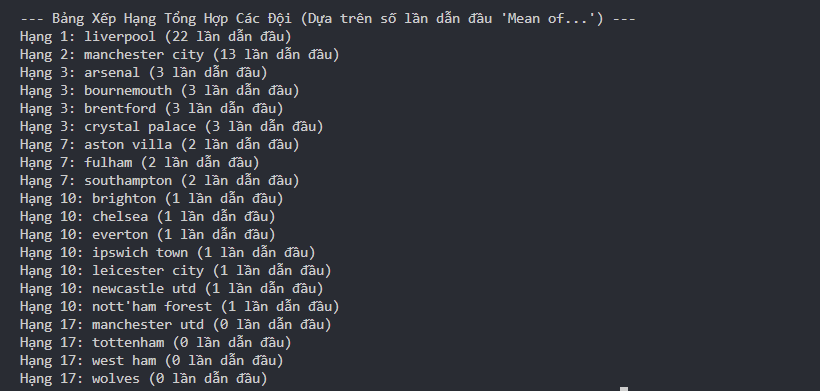
\includegraphics[width=0.8\textwidth]{output_2.4.2.png}
    \caption{Ví dụ bảng xếp hạng tổng hợp các đội.}
    \label{fig:overall_ranking}
\end{figure}

Dữ liệu thống kê cho thấy Liverpool là một tập thể thi đấu vượt trội và toàn diện, không chỉ nổi bật ở một vài khía cạnh mà duy trì phong độ ấn tượng trên hầu hết các chỉ số quan trọng của bóng đá hiện đại.
Họ sở hữu sức mạnh tấn công bùng nổ, khả năng kiểm soát bóng vượt trội cùng hệ thống phòng ngự vững chắc – tất cả tạo nên một cỗ máy thi đấu trơn tru và hiệu quả.
Trên thực tế họ đã giành được chức vô địch Premier League mùa giải 2024–2025 \textit{trước 4 vòng đấu} một cách đầy thuyết phục, với \textit{82 điểm} – bỏ xa đội nhì bảng Arsenal một khoảng cách an toàn.
Đây chính là minh chứng rõ ràng rằng, khi một đội bóng vận hành đúng hướng cả về chuyên môn lẫn chiến lược, sự áp đảo của họ sẽ được thể hiện rõ rệt qua các con số thống kê và kết quả trên sân cỏ.
% Hết chương 2

% Chương 3
\chapter{Phân cụm cầu thủ và giảm chiều dữ liệu với PCA}

\section{Phân cụm cầu thủ bóng đá sử dụng thuật toán k-means}

\subsection{Giới thiệu} 
Phân tích dữ liệu cầu thủ đóng vai trò quan trọng trong thể thao hiện đại, giúp các huấn luyện viên, nhà phân tích và người quản lý đưa ra quyết định sáng suốt.
Một trong những kỹ thuật phổ biến được sử dụng là thuật toán phân cụm K-means, nhằm mục đích phân chia một tập hợp các cầu thủ thành các nhóm (cụm) riêng biệt dựa trên sự tương đồng về các chỉ số thống kê của họ.
Phần này sẽ trình bày cách thuật toán K-means được áp dụng, đặc biệt tập trung vào việc xác định số lượng cụm tối ưu và bình luận về kết quả thu được từ việc chạy tệp mã nguồn \texttt{player\_clustering\_kmeans.py}.

\subsection{Lựa chọn phạm vi k để chạy thử nghiệm}
Việc chọn phạm vi $k$ để chạy thử nghiệm trong bài toán phân cụm cầu thủ (500 cầu thủ, 78 chỉ số) cần dựa trên các yếu tố lý thuyết, đặc điểm dữ liệu, và ngữ cảnh thực tiễn trong bóng đá.

\subsubsection*{Lý do chọn kmin = 3}
\begin{itemize}
    \item \textbf{Yêu cầu tối thiểu để có phân cụm có ý nghĩa:}
    \begin{itemize}
        \item k=1: không tạo ra cụm (tất cả dữ liệu thuộc cùng một nhóm), không có giá trị phân tích.
        \item k=2: chỉ chia dữ liệu thành hai nhóm, thường quá đơn giản cho dữ liệu khoảng 78 chỉ số (chỉ phân biệt thô sơ như "tấn công" và "phòng ngự").
    
        \item k=3: điểm khởi đầu hợp lý để phản ánh các vai trò cơ bản trong bóng đá, ví dụ: thủ môn, cầu thủ phòng ngự, cầu thủ tấn công.
    \end{itemize}
    \item \textbf{Phù hợp với số lượng mẫu:}
    \begin{itemize}
        \item Với 500 cầu thủ, k=3 tạo ra các cụm trung bình $500/3 \approx 167$ cầu thủ/cụm, đủ lớn để mang ý nghĩa thống kê.
    \end{itemize}
\end{itemize}
\textbf{Kết luận:} kmin=3 là điểm khởi đầu hợp lý.

\subsubsection*{Lý do chọn kmax = 15}
\begin{itemize}
    \item \textbf{Dựa trên số lượng mẫu (khoảng 500 cầu thủ):}
    \begin{itemize}
        \item Mỗi cụm nên có ít nhất 20–50 mẫu để đảm bảo ý nghĩa thống kê:
        \begin{itemize}
            \item Nếu mỗi cụm có tối thiểu 20 cầu thủ: $k = 500/20 = 25$
            \item Nếu mỗi cụm có tối thiểu 50 cầu thủ: $k = 500/50 = 10$. 
        \end{itemize}
        \item Để các cụm không quá nhỏ, kmax nên nằm trong khoảng 10–25. Tuy nhiên, cần cân nhắc thêm ngữ cảnh.
    \end{itemize}
    \item \textbf{Ngữ cảnh bóng đá:}
    \begin{itemize}
        \item Số vai trò/phong cách chơi trong bóng đá hiếm khi vượt quá 15–20 (ví dụ: thủ môn, hậu vệ trung tâm, hậu vệ cánh, tiền vệ phòng ngự, tiền vệ tấn công, tiền vệ cánh, trung phong, tiền đạo lùi, v.v.).
        \item k=15 đủ để bao quát các vai trò chi tiết mà không vượt quá giới hạn thực tế.
    \end{itemize}
    \item \textbf{Kinh nghiệm thực tiễn:}
    \begin{itemize}
        \item Trong các bài toán phân cụm tương tự, kmax=15 thường đủ để bao quát các điểm khuỷu tay (thường xuất hiện trong khoảng k=4 đến k=10), tránh lãng phí tài nguyên tính toán.
    \end{itemize}
\end{itemize}
\textbf{Kết luận:} kmax=15 là ngưỡng hợp lý.
Phạm vi k từ 3 đến 15 là hợp lý: kmin=3 tạo cụm cơ bản (167 cầu thủ/cụm), kmax=15 bao quát vai trò chi tiết (33 cầu thủ/cụm), phù hợp với dữ liệu, ngữ cảnh bóng đá, và điểm khuỷu tay thường trong k=4 đến k=10.

\subsection{Xác định số lượng cụm tối ưu (K) và Quy trình thực thi}
\textbf{Ý tưởng chính:} Để xác định số lượng cụm (K) tối ưu cho việc phân nhóm cầu thủ, em đã áp dụng phương pháp Elbow.
Quy trình này bắt đầu bằng việc thử nghiệm thuật toán K-Means với một loạt các giá trị K tiềm năng, cụ thể là từ 3 đến 15 cụm.
Đối với mỗi giá trị K, chỉ số WCSS (Within-Cluster Sum of Squares - tổng bình phương khoảng cách từ mỗi điểm dữ liệu đến tâm cụm của nó) được tính toán.
WCSS là một thước đo về độ chặt chẽ của các cụm; giá trị WCSS thấp hơn cho thấy các điểm dữ liệu trong cùng một cụm gần nhau hơn.
Sau đó, các giá trị WCSS này được trực quan hóa trên một biểu đồ đường, với số lượng cụm (K) trên trục hoành và WCSS tương ứng trên trục tung.
Điểm "khuỷu tay" (elbow point) trên biểu đồ, nơi mà việc tăng thêm số cụm K không còn dẫn đến sự sụt giảm đáng kể của WCSS, được xác định là giá trị K tối ưu.
Dựa trên phân tích biểu đồ Elbow, một giá trị K phù hợp đã được lựa chọn.
Cuối cùng, thuật toán K-Means được thực thi lại với số cụm K tối ưu này để tiến hành phân chia các cầu thủ vào các nhóm tương ứng, qua đó mỗi cầu thủ được gán vào một cụm dựa trên sự tương đồng về các chỉ số thống kê.

\subsubsection*{Cấu hình và khởi tạo}
\begin{itemize}
    \item \textbf{Import thư viện:} Nạp các thư viện cần thiết như \texttt{pandas}, \texttt{numpy}, \texttt{os}, \texttt{sklearn.cluster.KMeans} (cho thuật toán K-Means), \texttt{sklearn.preprocessing.StandardScaler} (để chuẩn hóa dữ liệu), \texttt{sklearn.impute.SimpleImputer} (để xử lý giá trị thiếu), \texttt{matplotlib.pyplot} và \texttt{seaborn} (để vẽ biểu đồ).
    \item \textbf{Định nghĩa hằng số cấu hình:}
    \begin{itemize}
        \item \texttt{PLAYER\_COL}: Tên cột chứa tên cầu thủ (mặc định là 'Name').
        \item \texttt{CSV\_RELATIVE\_PATH}: Đường dẫn tương đối đến tệp CSV chứa dữ liệu cầu thủ (mặc định là \texttt{../problem\_1/results1.csv}).
        \item \texttt{script\_dir}: Lấy đường dẫn thư mục hiện tại của script.
        \item \texttt{output\_folder\_name}: Tên thư mục để lưu kết quả phân tích (mặc định là \texttt{kmeans\_analysis\_results}).
        \item \texttt{OUTPUT\_DIR}: Tạo đường dẫn tuyệt đối đến thư mục lưu kết quả.
    \end{itemize}
    \item \textbf{Định nghĩa hàm trợ giúp \texttt{ensure\_dir(path: str)}:} Hàm này đảm bảo rằng một thư mục tồn tại tại đường dẫn được cung cấp; nếu không, nó sẽ tạo thư mục đó.
\end{itemize}

\subsubsection*{Hàm chính \texttt{cluster\_players\_kmeans(csv\_path: str, player\_col: str, max\_k: int = 10)}}
\begin{itemize}
    \item \textbf{Nạp Dữ liệu:}
    \begin{itemize}
        \item Xác định đường dẫn tuyệt đối đến tệp CSV.
        \item Đọc dữ liệu từ tệp CSV vào một DataFrame của \texttt{pandas}.
    \end{itemize}
    \item \textbf{Chuẩn bị Dữ liệu:}
    \begin{itemize}
        \item Chọn các cột số: Xác định và chọn tất cả các cột trong DataFrame có kiểu dữ liệu là số để sử dụng làm đặc trưng cho việc phân cụm (loại bỏ cả cột ‘Age’ để làm cho các cụm phản ánh rõ ràng hơn sự tương đồng về kỹ năng, phong cách chơi hoặc vai trò chiến thuật, thay vì bị ảnh hưởng bởi yếu tố giai đoạn sự nghiệp của cầu thủ).
        \item Xử lý giá trị thiếu (NaN): Sử dụng \texttt{SimpleImputer} để thay thế bất kỳ giá trị thiếu nào trong các cột số đã chọn bằng giá trị trung bình của cột tương ứng.
        \item Chuẩn hóa Dữ liệu: Sử dụng \texttt{StandardScaler} để chuẩn hóa các đặc trưng số. Việc này đảm bảo rằng tất cả các đặc trưng đều có cùng một thang đo, điều này rất quan trọng đối với các thuật toán dựa trên khoảng cách như K-Means.
    \end{itemize}
    \item \textbf{Xác định số cụm tối ưu (K) bằng phương pháp Elbow:}
    \begin{itemize}
        \item Khởi tạo một danh sách \texttt{wcss} (Within-Cluster Sum of Squares - tổng bình phương khoảng cách nội cụm).
        \item Lặp qua một phạm vi các giá trị K có thể (từ 3 đến 15).
        \item Với mỗi giá trị K:
        \begin{itemize}
            \item Tạo một mô hình K-Means (\texttt{KMeans}) với số cụm là K, phương thức khởi tạo \texttt{'k-means++'}, \texttt{n\_init='auto'} (để tự động chọn số lần chạy với các hạt giống tâm cụm khác nhau), và \texttt{random\_state=42} (để đảm bảo kết quả có thể tái tạo).
            \item Huấn luyện mô hình K-Means trên dữ liệu đã chuẩn hóa.
            \item Lấy giá trị \texttt{inertia\_} (WCSS) của mô hình và thêm vào danh sách \texttt{wcss}.
        \end{itemize}
        \item Vẽ biểu đồ Elbow:
        \begin{itemize}
            \item Gọi hàm \texttt{ensure\_dir} để tạo thư mục đầu ra nếu chưa có.
            \item Tạo một biểu đồ đường (\texttt{plot}) với số lượng cụm (K) trên trục hoành và WCSS trên trục tung.
            \item Đặt tiêu đề, nhãn trục, và hiển thị lưới cho biểu đồ.
            \item Lưu biểu đồ Elbow dưới dạng tệp PNG vào thư mục \texttt{OUTPUT\_DIR}.
        \end{itemize}
        \item In ra thông báo hướng dẫn người dùng xem biểu đồ và chọn giá trị K tối ưu (điểm "khuỷu tay" trên biểu đồ, nơi WCSS bắt đầu giảm chậm lại).
    \end{itemize}
    \item \textbf{Nhận đầu vào K tối ưu từ người dùng:}
    \begin{itemize}
        \item Yêu cầu người dùng nhập số cụm K tối ưu dựa trên biểu đồ Elbow.
        \item Vòng lặp sẽ tiếp tục cho đến khi người dùng nhập một số nguyên hợp lệ trong phạm vi cho phép.
    \end{itemize}
    \item \textbf{Áp dụng K-means với K tối ưu:}
    \begin{itemize}
        \item Sau khi người dùng chọn K, tạo một mô hình K-Means cuối cùng với số cụm \texttt{optimal\_k} đã chọn.
        \item Huấn luyện mô hình K-Means cuối cùng này trên dữ liệu đã chuẩn hóa.
        \item Lấy nhãn cụm (cluster labels) được gán cho mỗi điểm dữ liệu (mỗi cầu thủ).
    \end{itemize}
    \item \textbf{Thêm nhãn cụm vào DataFrame gốc:}
    \begin{itemize}
        \item Tạo một bản sao của DataFrame gốc.
        \item Thêm một cột mới có tên \texttt{'Cluster'} vào bản sao này, chứa các nhãn cụm đã được gán.
    \end{itemize}
    \item \textbf{Phân tích và Lưu kết quả:}
    \begin{itemize}
        \item Phân tích tâm cụm:
        \begin{itemize}
            \item Tính toán tọa độ tâm của mỗi cụm trên thang đo đã chuẩn hóa (\texttt{final\_kmeans.cluster\_centers\_}).
            \item Chuyển đổi các tọa độ tâm này trở lại thang đo gốc bằng cách sử dụng \texttt{scaler.inverse\_transform()}.
            \item Tạo một DataFrame mới (\texttt{centroid\_df}) chứa các giá trị trung bình của các đặc trưng số cho mỗi cụm (ở thang đo gốc).
            \item In ra DataFrame tâm cụm này (đã làm tròn đến 2 chữ số thập phân).
            \item Lưu DataFrame tâm cụm vào một tệp CSV trong thư mục \texttt{OUTPUT\_DIR}.
        \end{itemize}
        \item Đếm số lượng cầu thủ trong mỗi cụm: In ra số lượng cầu thủ thuộc về mỗi cụm.
        \item Sắp xếp và Lưu DataFrame đã phân cụm:
        \begin{itemize}
            \item Sắp xếp DataFrame đã được gán nhãn cụm theo cột \texttt{'Cluster'}.
            \item Lưu DataFrame đã sắp xếp này vào một tệp CSV khác trong thư mục \texttt{OUTPUT\_DIR}.
        \end{itemize}
    \end{itemize}
    \item \textbf{Trả về} DataFrame đã phân cụm, đối tượng \texttt{scaler}, DataFrame các đặc trưng đã chuẩn hóa, và danh sách các cột số.
\end{itemize}

\subsubsection*{Khối thực thi chính (\texttt{if \_\_name\_\_ == '\_\_main\_\_':})}
\begin{itemize}
    \item \textbf{Gọi hàm phân cụm:} Gọi hàm \texttt{cluster\_players\_kmeans} với các tham số đã cấu hình (\texttt{CSV\_RELATIVE\_PATH}, \texttt{PLAYER\_COL}).
    \item \textbf{Lưu trữ các kết quả trả về} (DataFrame đã phân cụm, scaler, v.v.).
    \item \textbf{Hiển thị ví dụ cầu thủ từ mỗi cụm (nếu phân cụm thành công):}
    \begin{itemize}
        \item Kiểm tra xem \texttt{clustered\_data} có tồn tại không.
        \item Nếu có và danh sách \texttt{numeric\_cols\_list} không rỗng:
        \begin{itemize}
            \item Lặp qua từng ID cụm duy nhất (đã sắp xếp).
            \item In ra tiêu đề cho cụm đó.
            \item Lấy 5 cầu thủ đầu tiên (\texttt{head(5)}) từ cụm hiện tại.
            \item Chọn các cột để hiển thị: tên cầu thủ (\texttt{PLAYER\_COL}), tối đa 5 đặc trưng số đầu tiên, và cột \texttt{'Cluster'}.
            \item In ra thông tin của các cầu thủ mẫu này.
        \end{itemize}
    \end{itemize}
\end{itemize}

\subsection{Kết quả phân cụm K-means}


\begin{figure}[H]
    \centering
    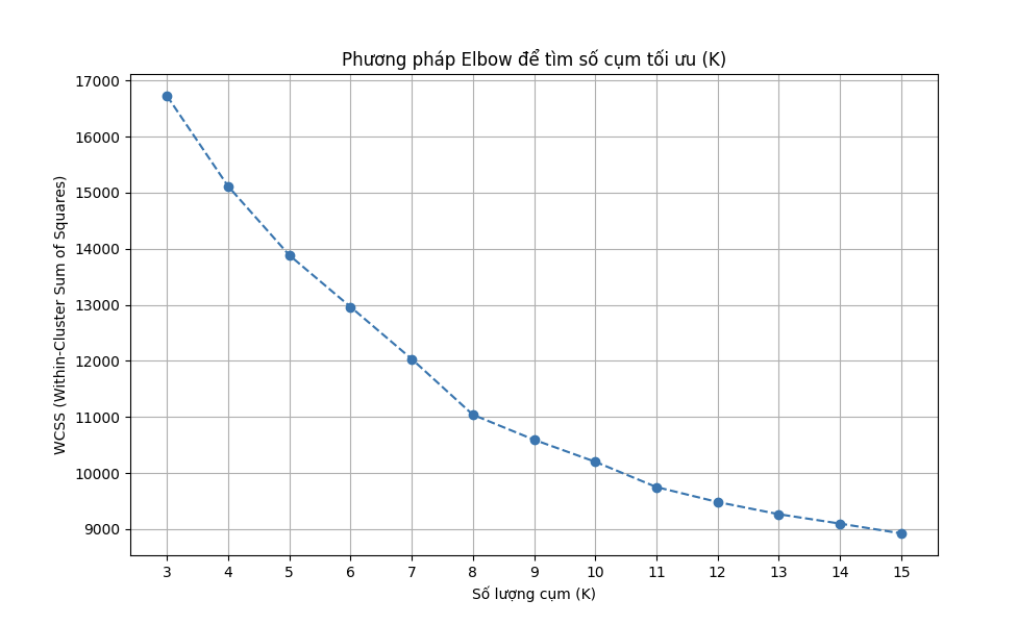
\includegraphics[width=\textwidth]{Elbow.png}
    \caption{Phương pháp Elbow để tìm số cụm tối ưu (K).}
    \label{fig:elbow_method}
\end{figure}

Biểu đồ Elbow cho thấy WCSS giảm mạnh từ k = 3 (17000) đến k = 6 (12000), sau đó giảm chậm từ k = 6 đến k = 15 (xuống 9000), đánh dấu k = 6 là điểm "cùi chỏ".
Lựa chọn k = 6 hợp lý vì nó cân bằng giữa chất lượng phân cụm (WCSS đã giảm đáng kể) và độ phức tạp mô hình, tránh tạo thêm cụm không cần thiết khi WCSS sau đó giảm không đáng kể.
Số lượng cầu thủ trong mỗi cụm sẽ được in ra màn hình.

\begin{figure}[H]
    \centering
    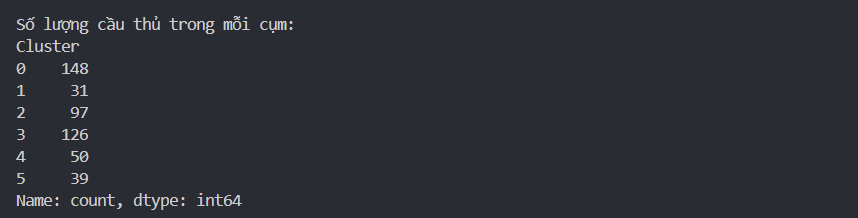
\includegraphics[width=\textwidth]{cluster.png}
    \caption{Số lượng cầu thủ trong mỗi cụm.}
    \label{fig:players_per_cluster}
\end{figure}


Các giá trị trung bình của từng chỉ số trong mỗi cụm được lưu vào tệp \texttt{cluster\_centroids.csv}, trong khi kết quả phân cụm chi tiết của từng cầu thủ được lưu vào tệp \texttt{player\_clusters\_sorted.csv}.
Dựa trên dữ liệu từ hai tệp này, em đã tiến hành phân tích đặc điểm nổi bật của từng cụm như sau:
\begin{itemize}
    \item \textbf{Cụm 0 (148 cầu thủ, ~30.1\%): Cầu thủ dự bị có vai trò phòng ngự hoặc Thủ môn.}
    \begin{itemize}
        \item Đặc trưng: Thời gian thi đấu thấp, đóng góp tấn công gần như không có (bàn thắng, kiến tạo, sút bóng, rê dắt tấn công đều ở mức thấp nhất trong các cụm).
        \item Hoạt động chủ yếu ở phần sân nhà (\texttt{Touches: Def Pen} cao), tỷ lệ chuyền ngắn/trung bình tốt (phù hợp với việc phát bóng hoặc luân chuyển an toàn).
        \item Số lượng: Cụm lớn nhất, cho thấy đây là nhóm phổ biến bao gồm các cầu thủ ít ra sân, chuyên gia phòng ngự sâu, hoặc có khả năng cao là các thủ môn của nhiều đội.
    \end{itemize}
    \item \textbf{Cụm 1 (31 cầu thủ, ~6.3\%): Tiền đạo mục tiêu/Sát thủ vòng cấm.}
    \begin{itemize}
        \item Đặc trưng: Ghi bàn (\texttt{Performance: goals}) và chỉ số bàn thắng kỳ vọng (\texttt{Expected: expected goals (xG)}) cao nhất tuyệt đối.
        \item Là điểm đến của các đường chuyền tấn công (\texttt{Progression: PrgR} cao nhất) và hoạt động nhiều nhất trong vòng cấm đối phương (\texttt{Touches: Att Pen} cao nhất).
        \item Khả năng tự phát triển bóng bằng chuyền (\texttt{Progression: PrgP}) thấp, củng cố vai trò người dứt điểm cuối cùng.
        \item Số lượng: Cụm nhỏ nhất, phản ánh sự chuyên biệt của các chân sút có hiệu suất cao và vai trò rõ ràng như vậy.
    \end{itemize}
    \item \textbf{Cụm 2 (97 cầu thủ, ~19.8\%): Tiền vệ trung tâm đa năng, cân bằng công thủ.}
    \begin{itemize}
        \itemĐặc trưng: Thời gian thi đấu cao. Dẫn đầu về các chỉ số phòng ngự quan trọng (ví dụ: \texttt{Tackles: Tkl} cao nhất, \texttt{Performance: Recov} cao nhất).
        \item Phát triển bóng hiệu quả từ tuyến hai (\texttt{Progression: PrgP} cao, \texttt{Expected: pass into final third (1/3)} nhiều) nhưng không phải là người kiến tạo chính yếu như Cụm 4 (kiến tạo, key passes thấp hơn đáng kể).
        \item Số lượng: Cụm lớn, cho thấy tầm quan trọng và sự phổ biến của các tiền vệ "xương sống", quán xuyến khu trung tuyến và kết nối lối chơi.
    \end{itemize}
    \item \textbf{Cụm 3 (126 cầu thủ, ~25.7\%): Cầu thủ dự bị có thiên hướng tấn công, tạo đột biến.}
    \begin{itemize}
        \item Đặc trưng: Thời gian thi đấu thấp nhất nhưng hiệu suất tấn công tính trên 90 phút rất đáng chú ý (đặc biệt \texttt{SCA: SCA90} - hành động tạo cú sút/90 phút - rất cao).
        \item Đóng góp phòng ngự thấp, cho thấy xu hướng được sử dụng để làm mới hàng công.
        \item Số lượng: Cụm lớn thứ hai, phản ánh việc các đội thường có nhiều phương án dự phòng để thay đổi cục diện trận đấu bằng những cầu thủ có khả năng tấn công.
    \end{itemize}
    \item \textbf{Cụm 4 (50 cầu thủ, ~10.2\%): Tiền vệ tấn công/Tiền đạo cánh kiến thiết chủ lực.}
    \begin{itemize}
        \item Đặc trưng: Dẫn đầu tuyệt đối ở hầu hết các chỉ số sáng tạo và kiến thiết lối chơi (\texttt{Performance: assists}, \texttt{Expected: key passes (KP)}, \texttt{SCA: SCA}, \texttt{GCA: GCA} đều cao nhất).
        \item Khả năng rê dắt (\texttt{Progression: PrgC}, \texttt{Take-Ons: Att}) và chuyền bóng phát triển tấn công (\texttt{Progression: PrgP}) vượt trội.
        \item Đồng thời cũng có khả năng ghi bàn tốt.
        \item Số lượng: Số lượng cầu thủ ở mức vừa phải, phản ánh vai trò quan trọng của các "nhạc trưởng" tấn công, những người thường là nhân tố chủ chốt nhưng không phải lúc nào cũng chiếm số đông trong một đội hình.
    \end{itemize}
    \item \textbf{Cụm 5 (39 cầu thủ, ~7.9\%): Trung vệ chủ chốt, có khả năng phát triển bóng từ tuyến dưới.}
    \begin{itemize}
        \item Đặc trưng: Thời gian thi đấu cao nhất. Thống trị các chỉ số phòng ngự chuyên biệt (\texttt{Blocks: Blocks}, \texttt{Blocks: Int}, \texttt{Aerial Duels: Won} đều cao nhất).
        \item Tỷ lệ chuyền bóng thành công cao nhất (\texttt{Total: Pass completion (Cmp\%)}) và khối lượng chuyền tịnh tiến từ sân nhà rất lớn (\texttt{Progression: PrgP}, \texttt{Expected: pass into final third (1/3)} cao), nhưng đóng góp tấn công trực tiếp (bàn thắng, kiến tạo) cực kỳ thấp.
        \item Số lượng: Cụm nhỏ, phù hợp với số lượng trung vệ đá chính thường có trong một đội bóng, đặc biệt là những người có bộ kỹ năng toàn diện cả phòng ngự lẫn phát triển bóng.
    \end{itemize}
\end{itemize}

\section{Trực quan hóa kết quả phân cụm cầu thủ bằng phương pháp phân tích thành phần chính (PCA)}

\subsection{Giới thiệu} 
Bài tập này nhằm mục tiêu trực quan hóa kết quả phân cụm các cầu thủ bằng cách sử dụng phương pháp Phân Tích Thành Phần Chính (PCA).
Dữ liệu đầu vào được lấy từ kết quả phân cụm trước đó, vốn được thực hiện bởi module \texttt{player\_clustering\_kmeans.py} dựa trên tập dữ liệu \texttt{results.csv}.
Đầu tiên, các đặc trưng của cầu thủ đã được chuẩn hóa và sau đó được giảm số chiều từ nhiều chiều xuống còn hai thành phần chính thông qua kỹ thuật PCA.
Quá trình này cho phép biểu diễn dữ liệu một cách trực quan trên mặt phẳng hai chiều, đồng thời vẫn giữ lại phần lớn thông tin quan trọng về sự khác biệt giữa các cụm.
Các cầu thủ sau đó được hiển thị trên biểu đồ phân tán 2D, với mỗi điểm dữ liệu được tô màu theo nhãn cụm đã được gán trước đó từ thuật toán K-Means.
Kết quả cuối cùng bao gồm biểu đồ trực quan hóa được lưu lại thành hình ảnh, cùng với bộ dữ liệu đã giảm chiều và nhãn phân cụm đi kèm, giúp thuận tiện cho việc phân tích, đối chiếu và trình bày sau này.

\subsection{Quy trình thực hiện \newline
(Dựa trên script \texttt{pca\_visual\_kmeans.py})} 

Đoạn mã \texttt{pca\_visual\_kmeans.py} thực hiện các bước chính sau:
\begin{enumerate}[label=\textbf{Bước \arabic*:}, leftmargin=*]
    \item \textbf{Nạp và xử lý kết quả phân cụm K-Means:}
    \begin{itemize}
        \item Script gọi hàm \texttt{cluster\_players\_kmeans} từ module \texttt{player\_clustering\_kmeans.py}.
        \item Hàm này chịu trách nhiệm đọc dữ liệu cầu thủ từ \texttt{CSV\_RELATIVE\_PATH} (trỏ đến \texttt{../problem\_1/results.csv}), thực hiện phân cụm K-Means (bao gồm việc xác định số cụm \texttt{optimal\_k} và chuẩn hóa dữ liệu).
        \item Kết quả trả về bao gồm DataFrame \texttt{df\_clustered\_sorted} (chứa thông tin cầu thủ và nhãn cụm \texttt{Cluster} đã gán) và \texttt{features\_scaled\_df} (DataFrame các đặc trưng số đã được chuẩn hóa, là đầu vào cho PCA).
    \end{itemize}
    \item \textbf{Áp dụng phân tích thành phần chính (PCA):}
    \begin{itemize}
        \item Một đối tượng PCA từ thư viện \texttt{sklearn.decomposition} được khởi tạo với \texttt{n\_components=PCA\_COMPONENTS} (đặt bằng 2) để giảm dữ liệu xuống 2 chiều.
        \item Mô hình PCA được huấn luyện (fit) và áp dụng (transform) trên \texttt{features\_scaled\_df}.
        \item Kết quả là một mảng NumPy chứa tọa độ của mỗi cầu thủ trên 2 thành phần chính mới (PC1 và PC2).
        \item Tỷ lệ phương sai của dữ liệu gốc được giải thích bởi 2 thành phần chính này được tính toán và in ra màn hình.
    \end{itemize}
    \item \textbf{Trực quan hóa Kết quả phân cụm 2D:}
    \begin{itemize}
        \item Hai thành phần chính (PC1, PC2) được sử dụng làm trục X và Y cho biểu đồ.
        \item Sử dụng thư viện \texttt{seaborn} và \texttt{matplotlib}, một biểu đồ phân tán (scatter plot) được vẽ, trong đó mỗi điểm đại diện cho một cầu thủ.
        \item Các điểm được tô màu dựa trên cột \texttt{Cluster} từ \texttt{df\_clustered\_sorted}, giúp phân biệt các nhóm cầu thủ khác nhau.
        \item Biểu đồ được đặt tiêu đề, nhãn trục, chú giải (legend) và lưới (grid) để dễ đọc.
        \item Biểu đồ trực quan hóa này được lưu vào file ảnh có tên định dạng \texttt{kmeans\_pca\_\{optimal\_k\}\_clusters\_viz.png} trong thư mục \texttt{pca\_kmeans\_viz\_results}.
    \end{itemize}
    \item \textbf{Lưu dữ liệu cuối cùng:}
    \begin{itemize}
        \item Các tọa độ PC1, PC2 được ghép vào DataFrame \texttt{df\_clustered\_sorted} để tạo thành \texttt{df\_pca\_clustered}.
        \item DataFrame này, chứa thông tin cầu thủ, nhãn cụm K-Means, và hai thành phần chính PCA, được lưu vào file CSV có tên định dạng \texttt{player\_clusters\_with\_pca\_\{optimal\_k\}.csv} trong cùng thư mục kết quả.
    \end{itemize}
\end{enumerate}

\subsection{Kết quả và nhận xét} % Tài liệu gốc có 3.3.3.

\begin{figure}[H]
    \centering
    % Thay 'pca_kmeans_visualization.png' bằng tên file ảnh thực tế của bạn
    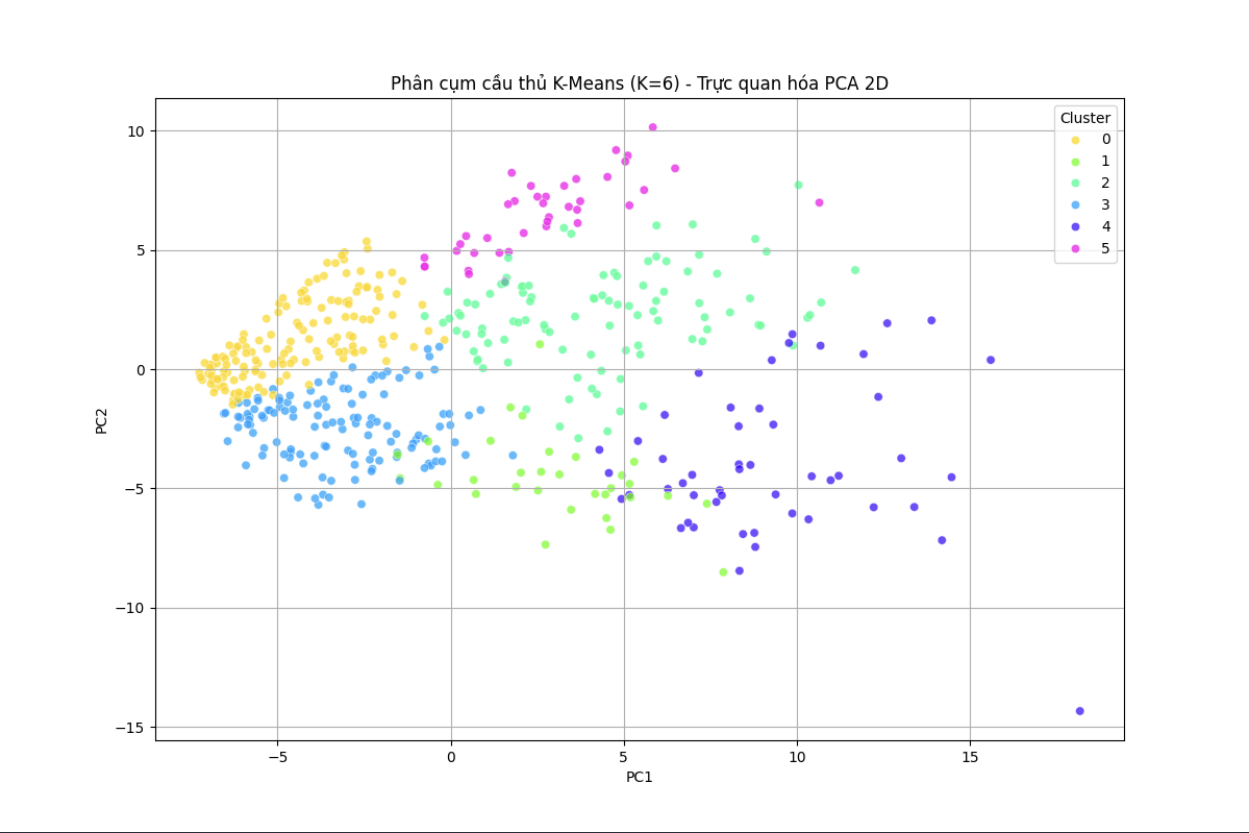
\includegraphics[width=\textwidth]{pca_kmeans.png}
    \caption{Phân cụm cầu thủ K-Means (K=6) - Trực quan hóa PCA 2D.}
    \label{fig:pca_kmeans_viz}
\end{figure}

\textbf{Nhận xét về biểu đồ PCA:}
Tỷ lệ phương sai được giải thích bởi 2 thành phần chính (PC1 và PC2): 0.6499 (tức là 64.99\%).
Điều này cho thấy hai thành phần chính đầu tiên giải thích được khoảng 65\% tổng phương sai trong dữ liệu, còn lại 35\% thông tin nằm ở các thành phần khác.
Biểu đồ cho thấy các cụm được phân chia khá rõ ràng, nhưng có một số vùng chồng lấn giữa các cụm, đặc biệt ở khu vực trung tâm (gần giao điểm PC1 = 0, PC2 = 0).
Điều này cho thấy một số cầu thủ có đặc điểm tương đối giống nhau giữa các cụm, có thể do các thông số thống kê của họ (ví dụ: số bàn thắng, kiến tạo, hoặc các chỉ số phòng ngự) không khác biệt lớn.
\begin{itemize}
    \item Cụm 0 (màu vàng) tập trung chủ yếu ở góc trái trên của biểu đồ (PC1 âm, PC2 dương), có thể đại diện cho một nhóm cầu thủ với các đặc điểm riêng biệt (ví dụ: các hậu vệ hoặc thủ môn, dựa trên dữ liệu CSV, vì họ có xu hướng không ghi bàn và tham gia nhiều vào phòng ngự).
    \item Cụm 1 (màu xanh lá nhạt) nằm ở phía dưới bên phải (PC1 dương, PC2 âm), có thể là nhóm các tiền đạo hoặc cầu thủ tấn công ghi bàn nhiều (như Alexander Isak, Yoane Wissa trong cụm này).
    \item Cụm 2 (màu xanh lam) phân bố rộng ở khu vực trung tâm và bên phải, có thể là các tiền vệ hoặc hậu vệ cánh với vai trò cân bằng giữa tấn công và phòng ngự (như Alexis Mac Allister, Andrew Robertson).
    \item Cụm 3 (màu xanh lam nhạt) tập trung ở góc trái dưới (PC1 âm, PC2 âm), có thể là các cầu thủ trẻ hoặc dự bị với ít thời gian thi đấu và ít đóng góp vào các chỉ số tấn công (như Abdul Fatawu Issahaku, Adam Lallana).
    \item Cụm 4 (màu tím) nằm ở phía bên phải (PC1 dương), có thể là các cầu thủ tấn công hoặc cánh với nhiều pha đi bóng và tham gia tấn công (như Alejandro Garnacho, Adama Traoré).
    \item Cụm 5 (màu hồng) phân bố rải rác nhưng tập trung ở khu vực PC2 dương lớn, có thể là các trung vệ hoặc cầu thủ phòng ngự với chỉ số phòng ngự cao (như Virgil van Dijk, Wout Faes).
\end{itemize}

\subsection{Kết luận} % Tài liệu gốc có 3.3.4.
Script \texttt{pca\_visual\_kmeans.py} thực hiện thành công yêu cầu trực quan hóa kết quả phân cụm K-Means của cầu thủ bằng cách sử dụng PCA để giảm chiều dữ liệu xuống 2D.
Kết quả là một biểu đồ phân tán 2D và một bộ dữ liệu mới kèm theo tọa độ PCA, cho phép đánh giá trực quan ban đầu về sự phân tách của các cụm.
Mặc dù phương pháp này có những hạn chế nhất định liên quan đến mất mát thông tin, nó vẫn là một công cụ hữu ích trong bộ công cụ phân tích dữ liệu để khám phá và trình bày kết quả phân cụm một cách dễ hiểu hơn.
% Hết chương 3

% Chương 4
\chapter{Thu thập giá trị chuyển nhượng và xây dựng mô hình ước tính giá trị cầu thủ}

\section{Thu thập và xử lý giá trị chuyển nhượng cầu thủ mùa giải 2024-2025}

\subsection{Giới thiệu}
Phần báo cáo này trình bày quy trình thu thập dữ liệu giá trị chuyển nhượng của các cầu thủ bóng đá cho mùa giải 2024-2025 từ trang web \url{https://www.footballtransfers.com}.
Quá trình này tập trung vào việc lấy thông tin của những cầu thủ có thời gian thi đấu thực tế lớn hơn 900 phút, dựa trên dữ liệu được cung cấp.
File mã nguồn chính là \texttt{transfer\_values\_2024-2025.py}.

\subsection{Cấu trúc thư mục và thư viện sử dụng}
\begin{itemize}
    \item Cấu trúc thư mục: Tổ chức gồm file code chính \texttt{transfer\_values\_2024-2025.py} và file cấu hình \texttt{config.json} trong thư mục gốc.
    \item Dữ liệu đầu vào được lấy từ thư mục \texttt{../problem\_1/}, và kết quả được lưu vào thư mục \texttt{OUTPUT/} (bao gồm \texttt{raw\_data.csv}, \texttt{player\_transfer\_values.csv}, \texttt{estimation\_data.csv}).
    \item {Thư viện chính sử dụng:} Python, \texttt{os}, \texttt{re}, \texttt{time}, \texttt{pandas}, \texttt{json}, \texttt{BeautifulSoup} (từ \texttt{bs4}), và \texttt{selenium} (cùng các modules con của nó).
\end{itemize}

\subsection{Quy trình thực hiện}
\begin{enumerate}[label=\textbf{Bước \arabic*:}, leftmargin=* , itemsep=1ex]
    \item \textbf{Tải cấu hình} \\
    Script bắt đầu bằng việc tải các thông số cấu hình từ file \texttt{config.json} thông qua hàm \texttt{load\_config}.
    File này chứa các đường dẫn quan trọng (ví dụ: \texttt{paths.part1\_results\_relative} cho file dữ liệu thời gian thi đấu, \texttt{paths.output\_folder} cho thư mục lưu kết quả), URL mục tiêu (\texttt{scraping.transfer\_url}), thông tin user-agent (\texttt{scraping.user\_agent} để mô phỏng trình duyệt), các CSS selector (trong \texttt{selectors}) để xác định vị trí các mẩu dữ liệu cụ thể trên trang web (như tên cầu thủ, ETV, nút "Next page"), và ngưỡng thời gian thi đấu tối thiểu (\texttt{processing.min\_minutes\_threshold}).

    \item \textbf{Thu thập dữ liệu (Web Scraping) - thực hiện trong hàm \texttt{scrape\_transfer\_data}:}
    \begin{itemize}[leftmargin=0em]
        \item Hàm \texttt{scrape\_transfer\_data} sử dụng Selenium để mở URL của trang danh sách cầu thủ (ví dụ: Premier League) được chỉ định trong \texttt{config.json}.
        \item Script duyệt qua từng trang trong danh sách cầu thủ.
        \item Selenium đợi cho các yếu tố cần thiết của trang, như bảng dữ liệu cầu thủ (\texttt{selectors.player\_table}), được tải hoàn tất trước khi tiến hành trích xuất.
        \item Đối với mỗi cầu thủ (mỗi hàng \texttt{selectors.player\_row} trong bảng), các thông tin sau được trích xuất dựa trên các CSS selector định nghĩa trong \texttt{config.json}:
        \begin{itemize}
            \item Tên cầu thủ (\texttt{selectors.player\_name})
            \item Tên đội (\texttt{selectors.team\_name})
            \item Giá trị chuyển nhượng ước tính (ETV - \texttt{selectors.etv})
            \item Tuổi (\texttt{selectors.age})
            \item Vị trí (\texttt{selectors.position})
            \item Kỹ năng (\texttt{selectors.skill})
            \item Tiềm năng (\texttt{selectors.potential})
        \end{itemize}
        \item Xử lý giá trị chuyển nhượng (ETV) ngay khi thu thập: Dữ liệu ETV thô (ví dụ: "€50.5m") được làm sạch và chuyển đổi sang đơn vị triệu Euro ngay tại bước này bằng hàm \texttt{clean\_transfer\_value}. Hàm này:
        \begin{itemize}
            \item Loại bỏ các ký tự tiền tệ (ví dụ: '€', '\$') và dấu phẩy.
            \item Nhận diện và xử lý các hậu tố 'm' (triệu) hoặc 'k' (nghìn) để quy đổi về giá trị số đầy đủ.
            \item Chuẩn hóa giá trị về đơn vị triệu (ví dụ 50.5).
            \item Nếu giá trị không hợp lệ, nó sẽ trả về \texttt{None}.
        \end{itemize}
        \item Tương tự, các giá trị số khác như Tuổi, Kỹ năng, Tiềm năng được trích xuất dưới dạng text và hàm \texttt{safe\_get\_numeric} cố gắng chuyển đổi chúng thành dạng số, xử lý dấu phẩy nếu có.
        \item Cơ chế "Chuyển nút" (Phân trang):
        \begin{itemize}
            \item Sau khi xử lý hết cầu thủ trên một trang, script tìm nút "Next page".
            \item Hàm \texttt{get\_next\_page\_button} được gọi, sử dụng \texttt{WebDriverWait} để chờ tối đa 5 giây cho đến khi nút "Next page" (được xác định bởi selector \texttt{selectors.next\_page\_enabled} từ \texttt{config.json}, ví dụ: \texttt{button.pagination\_next\_button:not([disabled])}) trở nên khả dụng và có thể click được. Selector này đảm bảo chỉ chọn nút đang hoạt động.
            \item Nếu không tìm thấy nút "Next page" hợp lệ (ví dụ, ở trang cuối cùng hoặc có lỗi tải trang), \texttt{get\_next\_page\_button} trả về \texttt{None}, và vòng lặp thu thập dữ liệu trên các trang sẽ kết thúc.
            \item Nếu nút được tìm thấy:
            \begin{itemize}
                \item Script thực hiện \sloppypar
                \texttt{driver.execute\_script("arguments[0].scrollIntoView(\{block: 'center'\});", next\_btn)} để cuộn nút vào giữa tầm nhìn của trình duyệt. Việc này giảm thiểu nguy cơ nút bị che bởi các phần tử khác và không thể click được.
                \item Một khoảng dừng ngắn ngẫu nhiên \sloppypar
                (\texttt{time.sleep(random.uniform(0.4, 0.8))}) được áp dụng.
                \item Script thử click nút bằng \texttt{next\_btn.click()}. Nếu xảy ra \sloppypar
                \texttt{ElementClickInterceptedException} \sloppypar (nghĩa là một phần tử khác đang che nút), script sẽ chuyển sang phương án dự phòng: thực hiện click bằng JavaScript với \texttt{driver.execute\_script("arguments[0].click();", next\_btn)}.
                \item Sau khi click thành công, một khoảng dừng dài hơn (\texttt{time.sleep(random.uniform(2.0, 3.5))}) được áp dụng để chờ trang mới tải hoàn tất trước khi tiếp tục vòng lặp.
            \end{itemize}
        \end{itemize}
        \item Sau khi hàm \texttt{scrape\_transfer\_data} hoàn tất việc duyệt qua tất cả các trang và thu thập thông tin của các cầu thủ vào một cấu trúc dữ liệu tạm thời (một dictionary trong Python), toàn bộ khối dữ liệu này (\texttt{scraped\_data}) sẽ được chuyển sang bước tiếp theo để xử lý, nơi nó sẽ được chuyển đổi thành DataFrame và lưu dưới dạng file dữ liệu thô (\texttt{raw\_data.csv}).
    \end{itemize}

    \item \textbf{Lọc dữ liệu dựa trên thời gian thi đấu:} 
    Đây là bước cốt lõi để đảm bảo chỉ những cầu thủ đáp ứng tiêu chí về thời gian thi đấu được giữ lại.
    \begin{itemize}[leftmargin=0em]
        \item \textbf{Lấy danh sách cầu thủ hợp lệ (\texttt{get\_valid\_players\_from\_part1}):} Hàm này đọc file CSV bên ngoài \texttt{results1.csv} (đường dẫn được khai báo trong \texttt{config.json} qua key \texttt{paths.part1\_results\_relative}).
        \item Từ file \texttt{results1.csv} này, script sẽ sử dụng chủ yếu hai cột quan trọng để lọc cầu thủ:
        \begin{itemize}
            \item Cột chứa tên cầu thủ, được xác định bởi giá trị của key \texttt{processing.part1\_player\_column} trong \texttt{config.json} (ví dụ: "Name").
            \item Cột chứa thời gian thi đấu của cầu thủ, được xác định bởi giá trị của key \texttt{processing.part1\_minutes\_column} trong \texttt{config.json} (ví dụ: "Playing Time: minutes").
        \end{itemize}
        \item Sau đó, thời gian thi đấu từ cột này sẽ được chuyển đổi sang dạng số và so sánh với ngưỡng \texttt{min\_minutes\_threshold} (900 phút) để tạo ra danh sách các tên cầu thủ "hợp lệ".
    \end{itemize}

    \item \textbf{Áp dụng bộ lọc vào dữ liệu đã thu thập}
    \begin{itemize}
        \item Trong hàm \texttt{process\_transfer\_data}, nếu danh sách cầu thủ hợp lệ (\texttt{valid\_player\_set}) không rỗng, script sẽ tiến hành lọc.
        \item Một cột tạm thời \texttt{Player\_Normalized} được tạo trong \texttt{df\_raw} bằng cách chuẩn hóa cột 'Player' (loại bỏ khoảng trắng thừa).
        \item \texttt{df\_raw} sau đó được lọc để chỉ giữ lại những hàng mà giá trị trong cột \texttt{Player\_Normalized} có trong \texttt{valid\_player\_set}.
        \item Cột tạm thời \texttt{Player\_Normalized} được xóa sau khi lọc.
        \item Nếu không có danh sách cầu thủ hợp lệ nào được tìm thấy từ file CSV đầu vào (ví dụ: file không tồn tại, không có cầu thủ nào thỏa mãn ngưỡng), thì \texttt{df\_raw} (dữ liệu chưa lọc theo thời gian thi đấu) sẽ được trả về.
    \end{itemize}
\end{enumerate}

\subsection{Kết quả}

\begin{figure}[H]
    \centering
    % Thay 'player_transfer_values_example.png' bằng tên file ảnh thực tế của bạn
    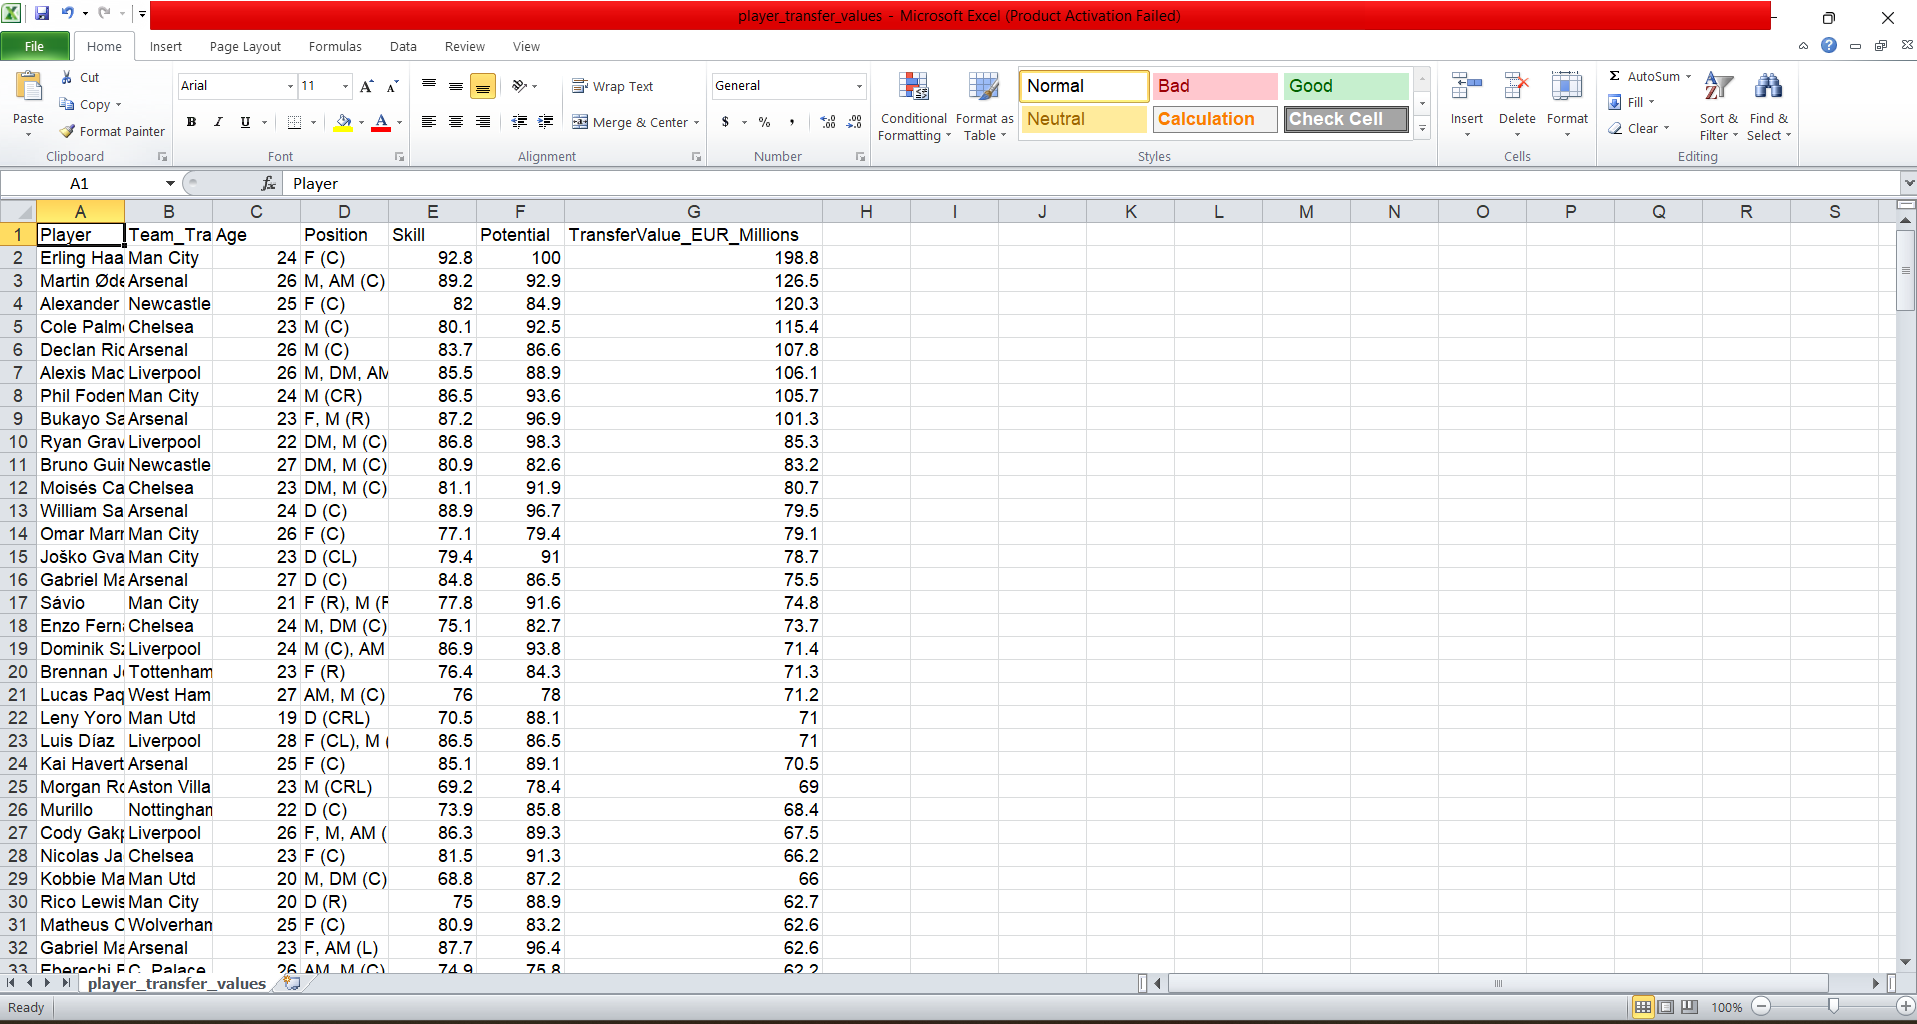
\includegraphics[width=\textwidth]{player_values.png}
    \caption{Ví dụ dữ liệu giá trị chuyển nhượng cầu thủ sau khi xử lý.}
    \label{fig:player_transfer_values}
\end{figure}

Quy trình tự động hóa thu thập và xử lý dữ liệu đã được triển khai thành công thông qua script \texttt{transfer\_values\_2024-2025.py} và file cấu hình \texttt{config.json}.
Kết quả của quá trình này là đã thu thập và lọc được thông tin chi tiết của \textbf{284 cầu thủ} có thời gian thi đấu thực tế trên 900 phút trong mùa giải 2024-2025 từ trang \texttt{footballtransfers.com}.
Dữ liệu thu được cho mỗi cầu thủ bao gồm các chỉ số quan trọng sau:
\begin{itemize}
    \item Đội (Team)
    \item Tuổi (Age)
    \item Vị trí (Position)
    \item Kỹ năng (Skill)
    \item Tiềm năng (Potential)
    \item Giá trị chuyển nhượng ước tính (TransferValue\_EUR\_Millions)
\end{itemize}
Toàn bộ dữ liệu này đã được lưu trữ trong các file output thông qua hàm \texttt{save\_data}:
\begin{itemize}
    \item \texttt{player\_transfer\_values.csv}: dữ liệu cuối cùng về giá trị chuyển nhượng của cầu thủ đã được xử lý và lọc
    \item \texttt{estimation\_data.csv}: chuẩn bị để sử dụng trong phần sau: dự đoán giá trị cầu thủ
\end{itemize}

\section{Xây dựng mô hình ước tính giá trị cầu thủ bóng đá}

\subsection{Giới thiệu}
Thị trường chuyển nhượng cầu thủ bóng đá là một lĩnh vực phức tạp và năng động, nơi việc định giá chính xác cầu thủ đóng vai trò quan trọng đối với các câu lạc bộ.
Phần báo cáo này trình bày phương pháp xây dựng một mô hình học máy để ước tính giá trị chuyển nhượng của cầu thủ, dựa trên các số liệu thống kê về hiệu suất, tiềm năng và các yếu tố khác.
Mục tiêu là đề xuất một quy trình có hệ thống từ thu thập dữ liệu, kỹ thuật đặc trưng, lựa chọn mô hình đến đánh giá và giải thích kết quả.
Biến mục tiêu là giá trị chuyển nhượng của cầu thủ, được biến đổi bằng hàm logarit (\texttt{Log\_TransferValue}) để ổn định phương sai và giảm tác động của các giá trị ngoại lai.

\subsection{Mô tả dữ liệu và tiền xử lý}
\subsubsection*{Nguồn dữ liệu và kết hợp}
\begin{itemize}
    \item \textbf{Nguồn dữ liệu:}
    \begin{itemize}
        \item Dữ liệu ước tính (\texttt{estimation\_data.csv}): Chứa các thông tin cơ bản và một số chỉ số ban đầu của cầu thủ.
        \item Dữ liệu kết quả (\texttt{results1.csv}): Có thể chứa các chỉ số hiệu suất chi tiết hơn từ một nguồn khác.
    \end{itemize}
    \item \textbf{Kết hợp dữ liệu:}
    \begin{itemize}
        \item Hai bộ dữ liệu được kết hợp (merged) dựa trên thông tin của cầu thủ và đội bóng.
        \item Tên đội bóng đã được chuẩn hóa để đảm bảo việc kết hợp chính xác (ví dụ: "B'mouth" thành "Bournemouth").
    \end{itemize}
    \item \textbf{Kết quả sau khi kết hợp:} (283, 85), nghĩa là có 283 mẫu (cầu thủ) và 85 đặc trưng ban đầu. Điều này được thực hiện trong hàm \texttt{load\_and\_merge\_data}.
\end{itemize}

\subsubsection*{Kỹ thuật đặc trưng (Feature Engineering)}

Mục tiêu của kỹ thuật đặc trưng là tạo ra các biến mới có ý nghĩa hơn từ dữ liệu thô, giúp mô hình học tốt hơn. Các bước chính bao gồm:
\begin{itemize}
    \item \textbf{Tạo vị trí chính (PrimaryPosition):} Từ cột \texttt{Position\_x} (có thể chứa nhiều vị trí), chỉ lấy vị trí đầu tiên làm vị trí chính của cầu thủ. Các giá trị thiếu hoặc không xác định được gán là 'Unknown'.
    \item \textbf{Chuẩn hóa và chuyển đổi kiểu dữ liệu số:} Các cột như 'Skill', 'Potential', 'Age\_x', 'Expected: expected goals (xG)', 'Expected: expected Assist Goals (xAG)', 'TransferValue\_EUR\_Millions' được chuyển đổi sang kiểu số. Các lỗi chuyển đổi (nếu có) được xử lý bằng cách gán giá trị \texttt{NaN}.
    \item \textbf{Tính toán các chỉ số hiệu suất trên 90 phút:}
    \begin{itemize}
        \item \texttt{GoalContrib\_per90}: Tổng số bàn thắng và kiến tạo trên 90 phút.
        \item \texttt{DefensiveActions\_per90}: Tổng số pha tắc bóng thành công (TklW) và chặn bóng (Int) trên 90 phút.
        \item \texttt{Progression\_per90}: Tổng số pha dẫn bóng và chuyền bóng tịnh tiến trên 90 phút.
    \end{itemize}
    \item \textbf{Chuẩn hóa các cột tỷ lệ phần trăm:} Các cột như 'Total: Pass completion (Cmp\%)', 'Aerial Duels: Won\%' được chuyển từ dạng chuỗi (ví dụ: "85\%") sang dạng số thập phân (ví dụ: 0.85).
    \item \textbf{Biến đổi biến mục tiêu:}
    \begin{itemize}
        \item Giá trị chuyển nhượng ('TransferValue\_EUR\_Millions') được đảm bảo không âm (các giá trị âm được cắt về 0).
        \item Tạo cột \texttt{Log\_TransferValue} bằng cách áp dụng hàm \texttt{np.log1p} (logarit tự nhiên của 1+x) cho \texttt{TransferValue\_EUR\_Millions}. Phép biến đổi này giúp:
        \begin{itemize}
            \item Giảm độ xiên của phân phối giá trị chuyển nhượng.
            \item Ổn định phương sai.
            \item Đảm bảo đầu vào của hàm logarit luôn dương, ngay cả khi giá trị chuyển nhượng là 0.
        \end{itemize}
    \end{itemize}
    \item \textbf{Kết quả sau kỹ thuật đặc trưng:} (283, 90), cho thấy có 5 đặc trưng mới được tạo ra hoặc các cột được xử lý. Quá trình này được thực hiện trong hàm \texttt{advanced\_feature\_engineering}.
\end{itemize}

\subsection{Lựa chọn đặc trưng và chuẩn bị dữ liệu cho mô hình}
\subsubsection{Lựa chọn Đặc trưng (Feature Selection)}

Không phải tất cả các đặc trưng được tạo ra đều hữu ích cho mô hình. Các đặc trưng sau đã được lựa chọn để đưa vào mô hình:
'Skill', 
'Potential', 
'Age\_x', 
'GoalContrib\_per90', 
'DefensiveActions\_per90', 
'Progression\_per90', 
'Expected: expected goals (xG)', 
'Expected: expected Assist Goals (xAG)', 
'Total: Pass completion (Cmp\%)', 
'Aerial Duels: Won\%', 
'PrimaryPosition\_enc'.

\textbf{Lý do lựa chọn (suy đoán dựa trên tên đặc trưng và kiến thức chung):}
\begin{itemize}
    \item \textit{Thuộc tính cá nhân:} 'Age\_x', 'Skill', và 'Potential' là các chỉ số nền tảng đánh giá chất lượng hiện tại, kinh nghiệm và tiềm năng phát triển tương lai của cầu thủ. Tuổi tác là một yếu tố quan trọng, thường có mối quan hệ phi tuyến với giá trị cầu thủ.
    \item \textit{Hiệu suất tấn công:} 'GoalContrib\_per90', 'Expected: expected goals (xG)', 'Expected: expected Assist Goals (xAG)' đo lường khả năng đóng góp trực tiếp vào mặt trận tấn công.
    \item \textit{Hiệu suất phòng ngự:} 'DefensiveActions\_per90' phản ánh đóng góp ở mặt trận phòng ngự.
    \item \textit{Khả năng phát triển bóng và kiểm soát:} 'Progression\_per90' và 'Total: Pass completion (Cmp\%)' cho thấy khả năng xử lý và phân phối bóng.
    \item \textit{Đặc điểm thể chất/kỹ năng cụ thể:} 'Aerial Duels: Won\%' quan trọng đối với một số vị trí.
    \item \textit{Yếu tố vị trí:} 'PrimaryPosition' là yếu tố quan trọng vì giá trị cầu thủ thường khác nhau đáng kể giữa các vị trí.
\end{itemize}

\subsubsection{Chuẩn bị dữ liệu}

Các bước chuẩn bị dữ liệu cuối cùng trước khi đưa vào mô hình, được thực hiện trong hàm \texttt{prepare\_model\_data}:
\begin{itemize}
    \item \textbf{Xử lý giá trị thiếu (Missing Values):} Đối với các đặc trưng số được chọn, giá trị thiếu được điền bằng giá trị trung bình của cột đó.
    \item \textbf{Chuẩn hóa đặc trưng số (Numerical Feature Scaling):} Các đặc trưng số được chuẩn hóa bằng \texttt{StandardScaler} (trừ các giá trị về trung bình 0 và phương sai 1). Điều này giúp các thuật toán nhạy cảm với thang đo (như XGBoost khi không dùng \texttt{tree\_method='hist'} hoặc các mô hình dựa trên khoảng cách) hoạt động hiệu quả hơn.
    \item \textbf{Mã hóa đặc trưng danh mục (Categorical Feature Encoding):} Đặc trưng \texttt{PrimaryPosition} được mã hóa bằng \texttt{LabelEncoder}. Mỗi vị trí duy nhất sẽ được gán một giá trị số nguyên.
    \item \textbf{Tạo ma trận đặc trưng (X) và vector mục tiêu (y):}
    \begin{itemize}
        \item X: Ma trận chứa các đặc trưng đã được xử lý (chuẩn hóa và mã hóa). Kích thước: (283, 10).
        \item y: Vector chứa biến mục tiêu \texttt{Log\_TransferValue}. Kích thước: (283,).
    \end{itemize}
    \item \textbf{Kiểm tra dữ liệu:} Đảm bảo ma trận X không rỗng và số lượng mẫu trong X khớp với y.
\end{itemize}

\subsection{Lựa chọn mô hình và huấn luyện}
\subsubsection{Lựa chọn Mô hình}

Mô hình được lựa chọn để ước tính giá trị cầu thủ là XGBoost (Extreme Gradient Boosting).
\textbf{Lý do lựa chọn mô hình XGBoost để ước tính giá trị cầu thủ:}
\begin{itemize}
    \item \textit{Khả năng nắm bắt mối quan hệ phức tạp và phi tuyến:} Giá trị cầu thủ được quyết định bởi sự tương tác đa chiều giữa nhiều yếu tố như tuổi tác, kỹ năng, tiềm năng và hiệu suất thi đấu. XGBoost, với cấu trúc dựa trên tập hợp các cây quyết định, xuất sắc trong việc tự động phát hiện và mô hình hóa các mối quan hệ phức tạp này (ví dụ: ảnh hưởng của tuổi không phải lúc nào cũng tuyến tính, hoặc tiềm năng có giá trị khác nhau ở các độ tuổi khác nhau) mà không đòi hỏi phải định nghĩa trước. Điều này cực kỳ quan trọng để phản ánh đúng bản chất của việc định giá cầu thủ.
    \item \textit{Hiệu suất dự đoán vượt trội và kiểm soát overfitting hiệu quả:} XGBoost nổi tiếng với khả năng đạt được độ chính xác cao trên dữ liệu dạng bảng. Thuật toán này tích hợp các cơ chế điều chuẩn (regularization L1, L2) và kỹ thuật tối ưu hóa (như \texttt{early\_stopping\_rounds} được sử dụng) giúp ngăn chặn mô hình trở nên quá phức tạp hoặc "học vẹt" dữ liệu huấn luyện. Kết quả là mô hình có khả năng tổng quát hóa tốt hơn trên dữ liệu mới, đảm bảo tính tin cậy của các dự đoán giá trị cầu thủ.
    \item \textit{Tối ưu hóa hiệu quả và cung cấp diễn giải về đặc trưng:} XGBoost được thiết kế để huấn luyện nhanh chóng, ngay cả trên các bộ dữ liệu tương đối lớn, nhờ vào các kỹ thuật như xử lý song song và phương pháp tạo histogram (\texttt{tree\_method='hist'}). Quan trọng hơn, nó cung cấp thông tin chi tiết về mức độ quan trọng của từng đặc trưng (ví dụ: \texttt{Age\_x}, \texttt{Skill}, \texttt{GoalContrib\_per90}), cho phép chúng ta hiểu rõ yếu tố nào có ảnh hưởng lớn nhất đến việc định giá. Điều này không chỉ giúp đánh giá mô hình mà còn mang lại những hiểu biết giá trị cho các nhà phân tích và quản lý bóng đá.
\end{itemize}

\subsubsection{Huấn luyện và Tối ưu hóa Tham số}

Quá trình huấn luyện được thực hiện trong hàm \texttt{train\_model}:
\begin{itemize}
    \item \textbf{Phân chia dữ liệu:} Dữ liệu (X, y) được chia thành tập huấn luyện (train set) và tập kiểm thử (test set) với tỷ lệ 80:20 (\texttt{test\_size=0.2}). \texttt{X\_train} có kích thước (226,11).
    \item \textbf{Tối ưu hóa siêu tham số (Hyperparameter Tuning):}
    \begin{itemize}
        \item Sử dụng \texttt{RandomizedSearchCV} để tìm bộ siêu tham số tốt nhất cho XGBoost.
        \item \texttt{RandomizedSearchCV} thử nghiệm một số lượng tổ hợp tham số ngẫu nhiên (\texttt{n\_iter=20}) từ một không gian tìm kiếm được định nghĩa trước (\texttt{param\_grid}).
        \item Đánh giá chéo (Cross-validation) với \texttt{cv=5} được sử dụng trong quá trình tìm kiếm để đảm bảo tính ổn định của kết quả.
        \item Chỉ số đánh giá được sử dụng trong quá trình tìm kiếm là \texttt{r2} (R-squared).
    \end{itemize}
    \item \textbf{Siêu tham số tốt nhất được tìm thấy:}
    \begin{itemize}
        \item subsample: 0.6
        \item n\_estimators: 1000
        \item max\_depth: 6
        \item learning\_rate: 0.05
        \item gamma: 0.5
        \item colsample\_bytree: 0.6
    \end{itemize}
    \item \textbf{Huấn luyện mô hình cuối cùng:} Mô hình XGBoost được huấn luyện lại trên toàn bộ tập huấn luyện (\texttt{X\_train}, \texttt{y\_train}) với bộ siêu tham số tốt nhất vừa tìm được. Có sử dụng \texttt{early\_stopping\_rounds=50} và \texttt{eval\_set=[(X\_test, y\_test)]} để theo dõi hiệu suất trên tập kiểm thử và dừng sớm nếu không có cải thiện, nhằm tránh overfitting.
    \item \textbf{Môi trường huấn luyện:} Quá trình huấn luyện mô hình XGBoost được thực hiện trên CPU.
\end{itemize}

\subsection{Đánh giá mô hình}

Mô hình được đánh giá trên toàn bộ dữ liệu đã qua xử lý (X, y).
\begin{itemize}
    \item \textbf{R² score (Hệ số xác định R bình phương = 0.880):} Điều này có nghĩa là khoảng 88.0\% sự biến thiên của \texttt{Log\_TransferValue} có thể được giải thích bởi các đặc trưng đầu vào của mô hình. Đây là một kết quả khá tốt, cho thấy mô hình có khả năng nắm bắt được các yếu tố quan trọng ảnh hưởng đến giá trị cầu thủ.
    \item \textbf{MSE (Mean Squared Error - Sai số toàn phương trung bình = 0.088):} Đây là giá trị trung bình của bình phương sai số giữa giá trị dự đoán và giá trị thực tế (trên thang đo logarit). Giá trị MSE càng nhỏ càng tốt.
\end{itemize}

\subsection{Phân tích và trực quan hóa kết quả}

Các biểu đồ trực quan hóa giúp hiểu rõ hơn về hiệu suất và hoạt động bên trong của mô hình.

\subsubsection*{Biểu đồ giá trị thực tế vs. giá trị dự đoán (\texttt{actual\_vs\_predicted.png})}
\begin{figure}[H]
    \centering
    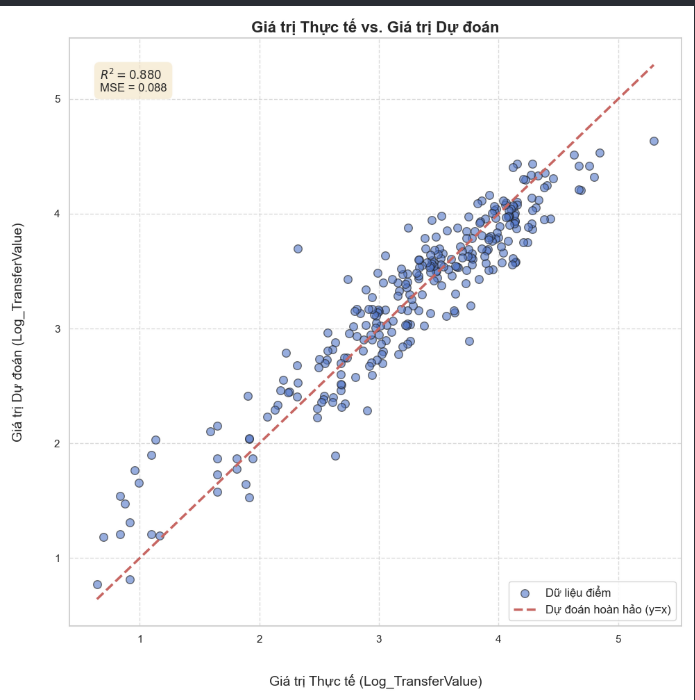
\includegraphics[width=\textwidth]{actual_vs_predicted.png}
    \caption{Biểu đồ giá trị thực tế vs giá trị dự đoán.}
    \label{fig:actual_vs_predicted}
\end{figure}

Dựa vào biểu đồ: Mô hình dự đoán giá trị cầu thủ \textbf{khá tốt}, thể hiện qua các điểm dữ liệu tập trung tương đối sát đường chéo (dự đoán hoàn hảo) và chỉ số R² cao (0.880).
Tuy nhiên, mô hình \textbf{vẫn có sai số} (MSE = 0.088, trên thang log), với một số điểm dự đoán lệch đáng kể so với giá trị thực tế, đặc biệt có thể ở các khoảng giá trị thấp và cao.

\subsubsection*{Biểu đồ Phần dư (\texttt{residual\_plot.png})}
\begin{figure}[H]
    \centering
    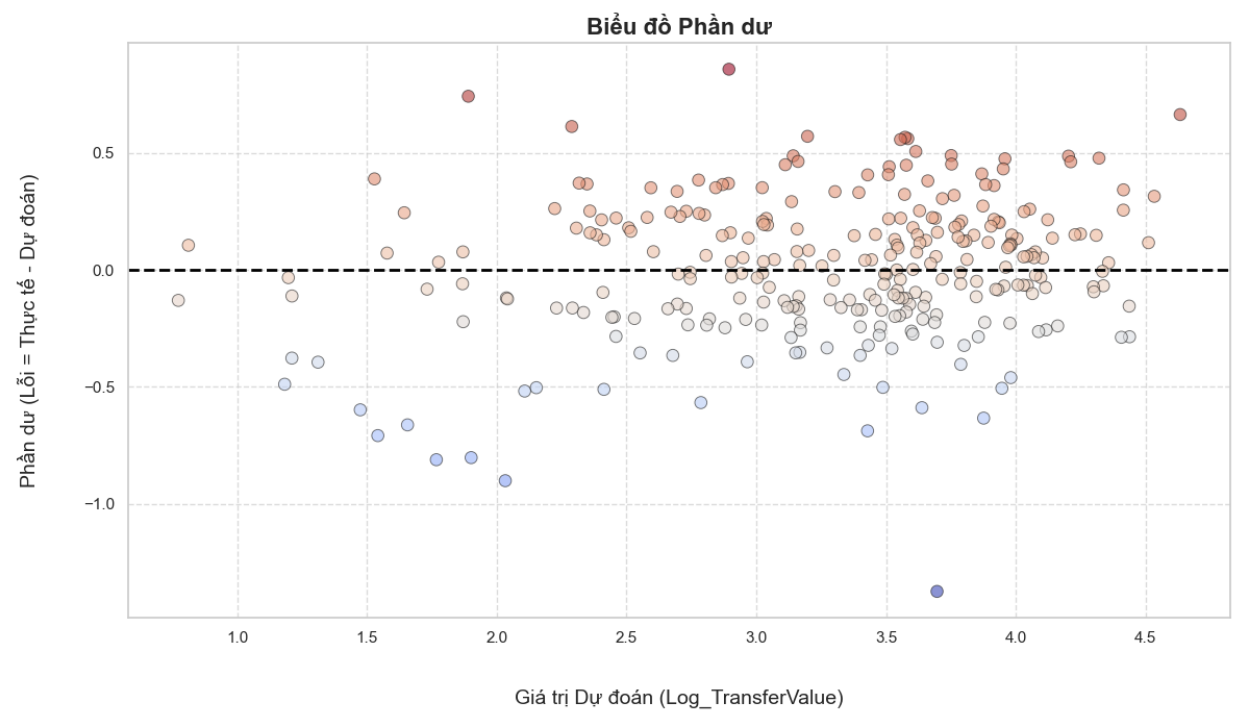
\includegraphics[width=\textwidth]{residual_plot.png}
    \caption{Biểu đồ Phần dư.}
    \label{fig:residual_plot}
\end{figure}

Biểu đồ phần dư cho thấy phần lớn các điểm phân bố gần đường 0 trên trục Phần dư, với một số ít điểm lệch đáng kể, đặc biệt ở các giá trị dự đoán cao (\texttt{Log\_TransferValue} lớn).
Điều này cho thấy mô hình XGBoost có hiệu quả tốt trong việc dự đoán giá trị cầu thủ, với độ chính xác cao ở phần lớn dữ liệu, nhưng có thể cần cải thiện đối với các trường hợp ngoại lệ hoặc giá trị cao.

\subsubsection*{Tầm quan trọng Đặc trưng của XGBoost (\texttt{xgb\_feature\_importance.png})}
\begin{figure}[H]
    \centering
    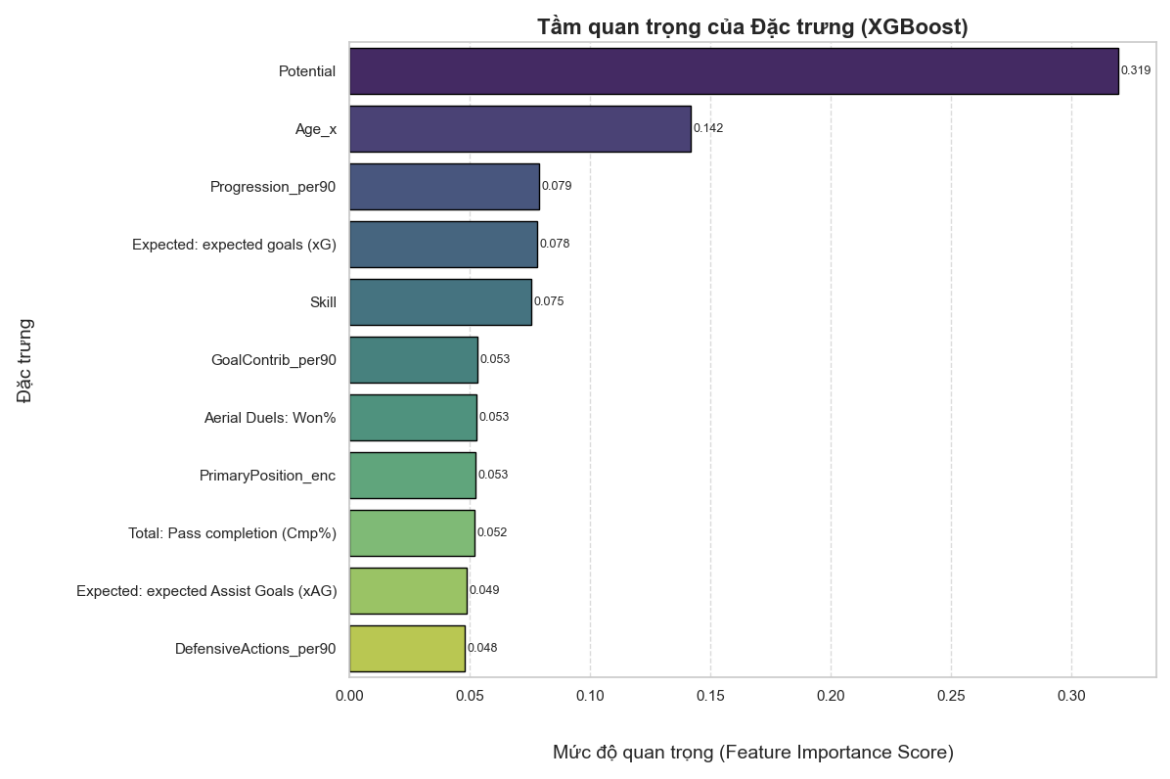
\includegraphics[width=\textwidth]{xgb_feature_importance.png}
    \caption{Biểu đồ Tầm quan trọng của Đặc trưng (XGBoost).}
    \label{fig:xgb_feature_importance}
\end{figure}

Biểu đồ Tầm quan trọng Đặc trưng của XGBoost cho thấy "Potential" là đặc trưng quan trọng nhất với điểm số 0.319, theo sau là "Age" (0.142).
Các đặc trưng như "Progression\_per90" (0.079), "Expected: expected goals (xG)" (0.078), và "Skill" (0.075) cũng có ảnh hưởng đáng kể.
Các đặc trưng khác như "DefensiveActions\_per90" (0.048) có mức độ quan trọng thấp hơn.
Điều này cho thấy mô hình phụ thuộc mạnh vào tiềm năng và tuổi của cầu thủ, đồng thời cân nhắc các chỉ số hiệu suất như tiến trình và kỹ năng.

\subsection{Kết luận và hướng phát triển}
\subsubsection*{Kết luận}
Phương pháp đề xuất đã xây dựng thành công một mô hình XGBoost để ước tính giá trị cầu thủ (biến đổi logarit) với hiệu suất khá tốt (R2=0.880). Quá trình này bao gồm các bước quan trọng từ kết hợp dữ liệu, kỹ thuật đặc trưng, lựa chọn và chuẩn bị đặc trưng, đến huấn luyện, tối ưu hóa và đánh giá mô hình. Các đặc trưng được lựa chọn như \texttt{Skill}, \texttt{Potential}, \texttt{Age} các chỉ số hiệu suất tấn công/phòng ngự trên 90 phút, và thông số về chuyền bóng/không chiến đã cho thấy khả năng đóng góp vào việc dự đoán giá trị. Việc sử dụng \texttt{RandomizedSearchCV} giúp tìm ra bộ siêu tham số tốt cho XGBoost. Các trực quan hóa cung cấp khả năng giải thích sâu sắc về hoạt động của mô hình.

\subsubsection*{Hướng phát triển}
\begin{itemize}
    \item \textbf{Đánh giá trên tập kiểm thử độc lập:} Để có đánh giá khách quan hơn về khả năng tổng quát hóa, cần đánh giá mô hình trên một tập dữ liệu kiểm thử hoàn toàn riêng biệt (không được sử dụng trong quá trình tối ưu hóa tham số).
    \item \textbf{Thử nghiệm các mô hình khác:} So sánh XGBoost với các thuật toán khác như LightGBM, CatBoost, hoặc các mô hình mạng neural đơn giản.
    \item \textbf{Kỹ thuật đặc trưng nâng cao hơn:}
    \begin{itemize}
        \item Xem xét các tương tác giữa các đặc trưng (ví dụ: \texttt{Skill} * \texttt{GoalContrib\_per90}).
        \item Thu thập thêm dữ liệu (ví dụ: thông tin về giải đấu, thông tin hợp đồng, thành tích đội bóng).
    \end{itemize}
    \item \textbf{Phân tích lỗi chi tiết:} Xem xét các trường hợp mà mô hình dự đoán sai nhiều nhất để hiểu rõ hơn về những hạn chế của mô hình.
    \item \textbf{Xử lý vấn đề mất cân bằng dữ liệu (nếu có):} Nếu giá trị cầu thủ phân bố rất không đều, có thể cần các kỹ thuật xử lý mất cân bằng.
    \item \textbf{Cập nhật mô hình định kỳ:} Giá trị cầu thủ và các yếu tố ảnh hưởng thay đổi theo thời gian, do đó mô hình cần được huấn luyện lại và cập nhật định kỳ với dữ liệu mới.
\end{itemize}
% Hết chương 4


\begin{thebibliography}{99}
\bibitem{XGBoostDocs}
XGBoost Developers. (2024). \textit{XGBoost Documentation (Release 3.0.0)}. 
Truy cập ngày 5 tháng 5 năm 2025, từ \url{https://xgboost.readthedocs.io/en/release_3.0.0/}

\bibitem{OngXuanHongBlogXGBoost}
Ông Xuân Hồng (2017, 21 tháng 12). \textit{XGBoost – thuật toán giành chiến thắng tại nhiều cuộc thi Kaggle}. 
Truy cập ngày 5 tháng 5 năm 2025, từ \url{https://ongxuanhong.wordpress.com/2017/12/21/xgboost-thuat-toan-gianh-chien-thang-tai-nhieu-cuoc-thi-kaggle/}

\bibitem{Li2022MLValue} 
Li, C., Kampakis, S., \& Treleaven, P. (2022). \textit{Machine Learning Modeling to Evaluate the Value of Football Players}. 
arXiv preprint arXiv:2207.11361. Truy cập ngày 5 tháng 5 năm 2025, từ \url{https://arxiv.org/pdf/2207.11361.pdf}



\end{thebibliography}

\end{document}
